% This must be in the first 5 lines to tell arXiv to use pdfLaTeX.
\pdfoutput=1

\documentclass[11pt]{article}

% EMNLP 2021 style
\usepackage{emnlp2021}

% Standard font packages
\usepackage{times}
\usepackage{latexsym}

% Character encoding
\usepackage[T1]{fontenc}
\usepackage[utf8]{inputenc}

% Improved layout
\usepackage{microtype}

% Math
\usepackage{amsmath}
\usepackage{amssymb}

% Tables and figures
\usepackage{booktabs}
\usepackage{graphicx}
\usepackage{subcaption}
\usepackage{multirow}
\usepackage{array}
\usepackage{tabularx}
\usepackage{adjustbox}
\usepackage{placeins}

% Cross-references
\usepackage[capitalize]{cleveref}

% Enumerate
\usepackage{enumitem}

\title{Acquiescence Is Not Personality:\\ Why Human Psychometric Instruments Fail on LLMs}

\author{Anonymous Authors}

\date{}

\begin{document}
\maketitle

\begin{abstract}
A growing body of work administers human personality questionnaires to LLMs and reports ``personality profiles.'' We ask a prior question: do these instruments actually measure anything meaningful in LLMs? We gave a 221-item battery (IPIP-NEO-120, SD3, ZKPQ-50-CC, EPQR-A) to 18 LLMs and subjected the 67,626 responses to standard psychometric validation. The core problem is acquiescence: LLMs tend to agree with every statement, regardless of direction. This single bias collapses the measurement. Agreeableness, the domain with the most reverse-coded items, yields $\alpha = 0.06$, because forward and reverse items pull in opposite directions under blanket agreement. The Big Five factor structure collapses from five to three factors. Inter-model variance is below 1\%: ``personality differences'' between models are effectively noise. The instruments are not measuring LLM personality; they are measuring the artifacts of alignment training.
\end{abstract}

\section{Introduction}

Can we measure the ``personality'' of a large language model? A growing body of work thinks so. Researchers administer human personality questionnaires to LLMs, compute scores, and report personality profiles \citep{miotto2023gpt3, bhandari2025evaluating, serapio2025psychometric, sorokovikova2024evaluating, lee2025trait}. Some even propose using LLMs as ``silicon samples'' to simulate survey respondents \citep{horton2023homo}.

But here is the problem. These instruments were designed for humans. A personality questionnaire is only valid for a population if it passes basic checks: internal consistency (Cronbach's $\alpha$), correct factor structure, convergent validity, and measurement invariance across subgroups \citep{cronbach1951coefficient, lord1968statistical}. Nobody checks these things before interpreting LLM personality scores.


\begin{figure}[t]
\centering

\includegraphics[width=\linewidth]{fig1_research_question_concept.png}
\caption{Conceptual framing of the research question. The paper does not assume that questionnaire scores are personality traits; it first asks whether the measurement conditions required for that interpretation hold for LLM responses.}
\label{fig:research-question}
\end{figure}
\FloatBarrier


The cracks are already showing. \citet{suhr2025challenging} found that LLMs endorse both forward-coded and reverse-coded items at the same time. \citet{tjuatja2023response} showed that LLM response biases in surveys differ systematically from human patterns. \citet{acerbi2024llm} and \citet{salecha2024llm} independently found that LLMs shift responses toward socially desirable endpoints by up to 1.2 human standard deviations. The instability goes deeper: \citet{pelet2025persistent} showed that reordering questions or changing conversation history produces different personality scores. \citet{huang2024reliability} found that scale reliability is highly sensitive to instructions and language. \citet{han2025personality} showed that self-reported personality in LLMs dissociates from actual behavior. Each of these findings chips away at the assumption that the instruments work. But each study looks at a different symptom. Nobody has run all the checks together, on the same data, to find the root cause.

That is what we do. Rather than profiling LLM personality, we ask a simpler question: do these instruments measure anything at all when given to LLMs? We administered a 221-item battery (the IPIP-NEO-120 \citep{johnson2014measuring}, the Short Dark Triad \citep{jones2014introducing}, the ZKPQ-50-CC \citep{aluja2006cross}, and the EPQR-A \citep{francis1992development}) to 18 LLMs across 17 role-conditioned prompts. Then we ran the same validation checks that psychometricians run before using any instrument on a new population. Every check failed. The cause is acquiescence: LLMs tend to agree with every statement, regardless of direction. This single bias explains why internal consistency collapses in reverse-heavy domains ($\alpha = 0.06$ for Agreeableness), why the Big Five factor structure shrinks to three, and why inter-model variance is below 1\%.

What makes our approach different from prior work is that we do not just report that LLM personality measurements are unreliable. We identify the specific mechanism (acquiescence), show which domains it destroys (those with many reverse-coded items), and demonstrate that the resulting scores reflect alignment artifacts rather than genuine traits. We also show a previously unreported asymmetry: normal personality items (IPIP) show positive acquiescence (agree with everything), while antisocial content (SD3) shows negative social desirability (reject dark traits). Two biases, one origin.

\section{Related Work}

\subsection{Personality Measurement in LLMs}

Researchers have administered personality questionnaires to LLMs and reported personality profiles \citep{miotto2023gpt3, serapio2025psychometric, bhandari2025evaluating, sorokovikova2024evaluating, lee2025trait, hagendorff2024machine}. But almost none of these studies check whether the instruments actually work on LLMs the way they work on humans. Benchmarks show systematic deviations between LLM and human responses \citep{xie2025aipsychobench}, temporal stability is limited \citep{bodroza2024personality}, and measurement invariance is assumed rather than tested \citep{suhr2025challenging}. \citet{chen2025humanizing} noted that most existing frameworks skip psychometric validation entirely.

\paragraph{Our contribution.}
Previous work asks ``what personality does this LLM have?'' and reports scores. We ask a different question: do these instruments measure anything meaningful at all when given to LLMs? Instead of profiling, we run the full set of standard psychometric validation checks---internal consistency, factor structure, convergent validity, reverse-item consistency, measurement invariance, and variance decomposition---on a single dataset covering 18 models and 221 items.

\subsection{Response Style and Acquiescence Bias}

Survey respondents do not always answer based on content alone. Acquiescence bias---agreeing with statements regardless of direction---is one of the most studied response styles \citep{paulhus1991response, lord1968statistical, baumgartner2007modeling}. It is especially damaging for instruments that rely on reverse-coded items. \citet{acerbi2024llm} and \citet{salecha2024llm} showed that LLMs also exhibit social desirability biases in Big Five surveys, and \citet{acquiescence2025emnlp} confirmed that acquiescence in LLMs is robust across languages.

\paragraph{Our contribution.}
These studies documented that acquiescence and social desirability exist in LLM responses. Our approach is different: we quantify the measurement damage they cause by decomposing the bias at item level, separating forward-coded and reverse-coded agree rates, and comparing across instruments with different content (normal personality vs.\ dark traits).

\subsection{Alignment Effects on LLM Behavior}

RLHF and safety training make LLMs more helpful and harmless, but also more homogeneous \citep{ouyang2022training, bai2022constitutional}. \citet{sharma2024sycophancy} showed that aligned models tend to echo user opinions even when wrong, and \citet{zheng2024agreeableness} linked Agreeableness scores to sycophancy in role-playing LLMs. \citet{wang2024aligning} argued that RLHF encodes a specific notion of acceptability that may override genuine variation.

\paragraph{Our contribution.}
These studies examined alignment effects on individual behaviors. We take a different angle: we test whether alignment produces a universal response style across model families via DIF analysis, and we quantify how far persona injection can push a model from its default behavior (Persona Separation Degree).

\section{Methodology}

\begin{figure*}[t]
\centering

\includegraphics[width=\textwidth]{fig2_methodology_pipeline.png}
\caption{Overview of the methodology. We administer a multi-instrument psychometric battery to LLMs, normalize the response matrix, and run standard validation checks before interpreting any score as evidence of personality.}
\label{fig:methodology-overview}
\end{figure*}

\subsection{Psychometric Instruments}

We administered a 221-item battery comprising four validated instruments (\cref{tab:instruments}). The \textbf{IPIP-NEO-120} \citep{johnson2014measuring} contains 120 Likert-5 items measuring the Big Five domains \citep{john1999bigfive, mccrae1992five} through 6 facets each, with 41 reverse-coded items. The \textbf{SD3} \citep{jones2014introducing} contains 27 Likert-5 items measuring Machiavellianism, Narcissism, and Psychopathy, with 5 reverse-coded items. The \textbf{ZKPQ-50-CC} \citep{aluja2006cross} contains 50 True/False items measuring 5 traits, with 12 reverse-coded items. The \textbf{EPQR-A} \citep{francis1992development} contains 24 Yes/No items measuring 4 traits, with 5 reverse-coded items.

\begin{table}[t]
\centering
\small
\caption{Psychometric instruments in the 221-item battery.}
\label{tab:instruments}
\begin{tabular}{lrrrr}
\toprule
Instrument & Items & Format & Domains & Rev. \\
\midrule
IPIP-NEO-120 & 120 & Likert-5 & 5 & 41 \\
SD3 & 27 & Likert-5 & 3 & 5 \\
ZKPQ-50-CC & 50 & T/F & 5 & 12 \\
EPQR-A & 24 & Y/N & 4 & 5 \\
\midrule
\textbf{Total} & \textbf{221} & 3 formats & \textbf{17} & \textbf{63} \\
\bottomrule
\end{tabular}
\end{table}

\subsection{Models and Administration Protocol}

We tested 18 LLMs spanning 7 model families (\cref{tab:models}): Anthropic (Claude Opus 4.6, Sonnet 4.6), OpenAI (GPT-5.5, GPT-5.2), DeepSeek (V3.2, V4-Flash, V4-Pro), Google (Gemini-3-Flash-Preview, Gemini-3.1-Flash-Lite, Gemini-3.1-Pro-Preview, Gemini-3-Pro-Preview), Alibaba (Qwen3-235B-A22B, Qwen3.5-122B-A10B, Qwen3.5-397B-A17B), Moonshot (Kimi-K2.5, Kimi-K2.6), MiniMax (M2.7), and Zhipu (GLM-4.6V).

\begin{table}[t]
\centering
\small
\caption{All 18 tested LLMs grouped by model family.}
\label{tab:models}
\begin{tabular}{l>{\centering\arraybackslash}p{5.2cm}}
\toprule
Family & Models \\
\midrule
Anthropic & Claude Opus 4.6, Sonnet 4.6 \\
OpenAI & GPT-5.5, GPT-5.2 \\
DeepSeek & V3.2, V4-Flash, V4-Pro \\
Google & Gemini-3-Flash, Gemini-3.1-Flash-Lite, Gemini-3.1-Pro, Gemini-3-Pro \\
Alibaba & Qwen3-235B-A22B, Qwen3.5-122B-A10B, Qwen3.5-397B-A17B \\
Moonshot & Kimi-K2.5, Kimi-K2.6 \\
MiniMax & M2.7 \\
Zhipu & GLM-4.6V \\
\bottomrule
\end{tabular}
\end{table}

Each model was tested under 17 conditions: a \textbf{Default} prompt (``Please answer the following personality questionnaire honestly.'') and 16 \textbf{MBTI persona} prompts, each assigning a specific MBTI type. All administrations used temperature = 0.7 with a single administration per model-condition pair. This yielded $18 \times 17 \times 221 = 67{,}626$ item-level responses.

\subsection{Analysis Pipeline}

We applied six checks that psychometricians use before trusting any instrument on a new population.

\paragraph{Internal consistency.}
We compute Cronbach's $\alpha$ per IPIP domain for each model, using the 17 persona conditions as observations. For a domain with $k$ items, let $X_{pi}$ be the scored response to item $i$ under persona $p$. Then:
\begin{equation}
\alpha = \frac{k}{k-1}\left(1 - \frac{\sum_{i=1}^{k} \mathrm{Var}(X_i)}{\mathrm{Var}\!\left(\sum_{i=1}^{k} X_i\right)}\right)
\label{eq:cronbach}
\end{equation}
We average $\alpha$ across the 18 models. Human benchmarks come from \citet{johnson2014measuring}.

\paragraph{Factor structure.}
Let $\mathbf{x}_j \in \mathbb{R}^{17}$ be the vector of domain scores for observation $j$ ($j = 1, \ldots, 306$). We standardize each domain to zero mean and unit variance, then compute the correlation matrix $\mathbf{R}$. We retain factors via the Kaiser criterion ($\lambda_i > 1$) and validate with parallel analysis: we permute each column of the data matrix independently, recompute eigenvalues, and repeat 500 times. A factor is retained only if its observed eigenvalue exceeds the 95th percentile of the permuted distribution. We extract factor loadings via eigendecomposition of $\mathbf{R}$ followed by varimax rotation.

\paragraph{Reverse-item consistency.}
For each domain that contains both forward-coded ($+$) and reverse-coded ($-$) items, we compute the Pairwise Inconsistency Rate (PIR). For Likert items, a forward-reverse pair $(f, r)$ is inconsistent when both responses fall on the same side of the midpoint:
{\small
\begin{equation}
\mathrm{PIR} = \frac{1}{|F|\,|R|} \sum_{f \in F}\sum_{r \in R} \mathbf{1}\!\bigl[\mathrm{sgn}(f{-}3) = \mathrm{sgn}(r{-}3)\bigr]
\label{eq:pir}
\end{equation}
}
where $F$ and $R$ are the sets of forward and reverse item responses, and the midpoint is 3 on the 1--5 scale. For binary items, inconsistency is $f = r$.

\paragraph{Variance decomposition.}
We normalize all responses to a common 0--1 scale: Likert scores via $x' = (x - 1)/4$, binary scores kept as-is. We then decompose the total sum of squares sequentially:
\begin{equation}
\begin{split}
\mathrm{SS}_{\mathrm{total}} &= \sum_{i}(y_i - \bar{y})^2 \\
&= \mathrm{SS}_{\mathrm{model}} + \mathrm{SS}_{\mathrm{domain}} \\
&\quad + \mathrm{SS}_{\mathrm{persona}} + \mathrm{SS}_{\mathrm{item}} + \mathrm{SS}_{\mathrm{resid}}
\end{split}
\label{eq:variance}
\end{equation}
where each component groups by the corresponding factor and computes the squared deviation of group means from the grand mean. We run this separately for Likert and binary scales.

\paragraph{Convergent validity.}
For each of 8 pre-specified construct pairs (e.g., IPIP Neuroticism vs.\ ZKPQ Neuroticism-Anxiety), we compute Pearson $r_p$ and Spearman $r_s$ across the 18 model-level means. A pair passes if the correlation sign matches the theoretical expectation.

\paragraph{Measurement invariance.}
For each model, let $\mathbf{d} \in \mathbb{R}^{120}$ be the vector of IPIP-NEO-120 parsed values under the Default persona, and $\mathbf{m}_k$ the same vector under MBTI persona $k$. We compute:
\begin{equation}
r_k = \mathrm{corr}(\mathbf{d},\, \mathbf{m}_k), \quad k = 1, \ldots, 16
\label{eq:invariance}
\end{equation}
Strong invariance requires $r_k > 0.8$ for all persona pairs. We report the mean $r$ across all $18 \times 16 = 288$ pairs.

\paragraph{Persona separation degree (PSD).}
To quantify how far a model can be pushed from its default personality by persona instructions, we define the Persona Separation Degree. Let $\mathbf{s}_{m,p} \in \mathbb{R}^{17}$ be the vector of domain mean scores for model $m$ under persona $p$. We z-score each domain across all $18 \times 17 = 306$ observations, yielding $\mathbf{z}_{m,p}$. For each model $m$ and persona $p \neq \mathrm{Default}$:
\begin{equation}
\mathrm{PSD}(m, p) = \frac{1}{\sqrt{17}}\left\| \mathbf{z}_{m,p} - \mathbf{z}_{m,\mathrm{Default}} \right\|_2
\label{eq:psd}
\end{equation}
Dividing by $\sqrt{17}$ normalizes to a per-dimension effect size in standard-deviation units. We report $\overline{\mathrm{PSD}}(m)$ (average malleability across 16 personas), $\mathrm{PSD}_{\max}(m)$ (peak plasticity), and $\mathrm{PSD}_{\mathrm{CV}}(m) = \sigma/\mu$ (differential responsiveness).

\paragraph{Persona steering diagnostics.}
PSD measures distance from Default, but distance alone does not tell us whether the model moves toward the requested persona. We therefore define two persona targets. The \textbf{empirical target} for model $m$ and persona $p$ is the leave-one-model-out centroid difference:
\begin{equation}
\mathbf{t}^{\mathrm{emp}}_{m,p} =
\bar{\mathbf{z}}_{-m,p} - \bar{\mathbf{z}}_{-m,\mathrm{Default}} .
\end{equation}
The \textbf{theoretical target} is a transparent MBTI-to-domain direction vector: E increases Extraversion/Sociability/Activity, N increases Openness, F increases Agreeableness and decreases dark/antagonistic traits, and J increases Conscientiousness while decreasing impulsivity. For each observed persona shift $\Delta_{m,p}=\mathbf{z}_{m,p}-\mathbf{z}_{m,\mathrm{Default}}$, we compute target adherence as $\cos(\Delta_{m,p}, \mathbf{t}_{m,p})$ and off-target leakage as the residual norm orthogonal to the target, divided by $\sqrt{17}$. We also classify each persona-conditioned profile to the nearest leave-one-model-out persona centroid, yielding a persona fidelity confusion matrix.

\paragraph{Cross-scale persona coherence and item plasticity.}
For overlapping constructs, we test whether persona-induced deltas move consistently across instruments: Extraversion (IPIP/EPQR/ZKPQ), Neuroticism (IPIP/EPQR/ZKPQ), Agreeableness versus antagonism (IPIP vs.\ SD3/ZKPQ), and Conscientiousness versus disinhibition (IPIP vs.\ ZKPQ/EPQR/SD3). We sign-align each construct and compute a coherence score, $|\overline{\Delta}|/\overline{|\Delta|}$, where 1 means all scales move in the same direction and 0 means they cancel. At the item level, we compute each item's mean absolute shift from Default and the rate at which forward/reverse item pairs move in theoretically opposite raw-score directions.

\section{Experiments and Results}

\subsection{Internal Consistency}

The most basic question: do items within a domain agree with each other? \cref{tab:cronbach} shows the answer. Extraversion, where only 17\% of items are reverse-coded, yields $\alpha = 0.92$. That is close to the human norm of 0.89. But Agreeableness, where 71\% of items are reverse-coded, yields $\alpha = 0.06$, essentially zero. The difference is not random. When a model agrees with both ``I am helpful'' and ``I am not helpful,'' the two items pull in opposite directions and the domain score falls apart. The more reverse-coded items a domain has, the worse its reliability. This is the fingerprint of acquiescence.

\begin{table}[t]
\centering
\small
\caption{Cronbach's $\alpha$ by IPIP domain: LLM vs.\ human norms. Mean$\pm$SD across $n{=}18$ models.}
\label{tab:cronbach}
\begin{tabular}{lrrr}
\toprule
Domain & LLM $\alpha$ & Human $\alpha$ & Gap \\
\midrule
Neuroticism & $0.749{\pm}0.186$ & 0.90 & $-0.151$ \\
Extraversion & $0.924{\pm}0.009$ & 0.89 & $+0.034$ \\
Openness & $0.193{\pm}0.140$ & 0.87 & $-0.677$ \\
Agreeableness & $0.060{\pm}0.363$ & 0.88 & $-0.820$ \\
Conscientiousness & $0.517{\pm}0.126$ & 0.90 & $-0.383$ \\
\bottomrule
\end{tabular}
\end{table}

\subsection{Default Personality Profiles}

Before diagnosing why the instruments fail, it helps to see what the raw profiles look like. \cref{fig:radar_default} shows the IPIP-NEO-120 scores under the Default prompt. All 18 models cluster in the same corner: high Agreeableness, high Conscientiousness, low Neuroticism. The inter-model range is narrowest for Agreeableness (0.92 on a 1--5 scale) and widest for Neuroticism (2.12). Alignment training compresses the socially desirable dimensions more tightly than the others. Every model looks like a ``nice, responsible, emotionally stable'' person.

\begin{figure}[t]
\centering
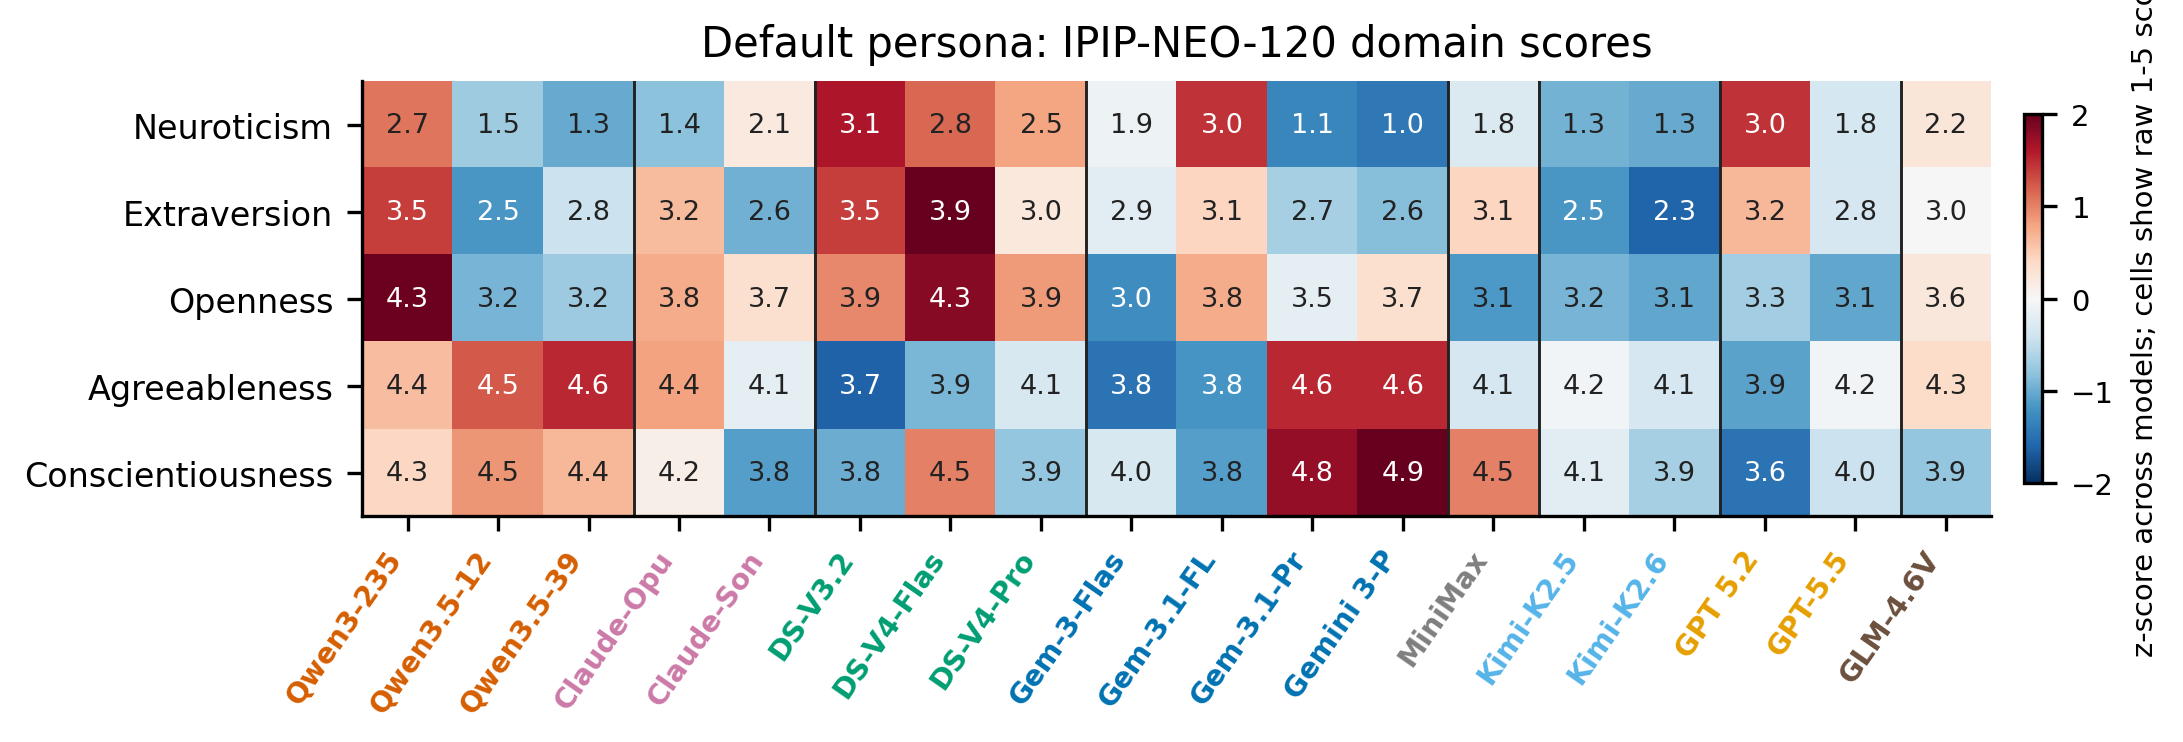
\includegraphics[width=\linewidth]{fig_heatmap_default.png}
\caption{Default persona IPIP-NEO-120 domain scores (z-scored heatmap). All 18 models cluster in a ``high A, high C, low N'' region. Inter-model range is narrowest for Agreeableness (0.92 on a 1--5 scale) and widest for Neuroticism (2.12).}
\label{fig:radar_default}
\end{figure}

\subsection{Factor Structure Collapse}

If acquiescence distorts individual domains, it should also distort the relationships between domains. \cref{tab:efa} shows the result. The Big Five does not survive. Instead of five factors, we get three.

Factor 1 captures Extraversion and Sociability (loadings: EPQR Extraversion $= 0.96$, ZKPQ Sociability $= 0.96$, IPIP Extraversion $= 0.94$). Factor 2 captures a merged Neuroticism-Agreeableness dimension (IPIP Neuroticism $= 0.72$, EPQR Neuroticism $= 0.91$, IPIP Agreeableness $= 0.90$). Factor 3 captures Conscientiousness versus Impulsivity (IPIP Conscientiousness $= -0.91$, ZKPQ ImpulsiveSS $= 0.84$, EPQR Psychoticism $= 0.88$). The merger of Neuroticism and Agreeableness is the smoking gun. In humans, these are orthogonal constructs. In LLMs, they collapse into a single ``socially desirable emotional stability'' factor because both are distorted by the same acquiescence pattern.

\begin{table}[t]
\centering
\small
\caption{EFA factor loadings (3-factor solution, $n{=}306$). Bold: $|l| > 0.5$. All 18 leave-one-model-out analyses recover exactly 3 factors.}
\label{tab:efa}
\begin{tabular}{lrrr}
\toprule
Domain & F1 & F2 & F3 \\
\midrule
IPIP N & $-$0.30 & \textbf{0.72} & 0.39 \\
IPIP E & \textbf{0.94} & 0.03 & 0.29 \\
IPIP O & $-$0.04 & \textbf{0.55} & \textbf{0.58} \\
IPIP A & 0.05 & \textbf{0.90} & $-$0.22 \\
IPIP C & $-$0.00 & $-$0.04 & $\mathbf{-}$0.91 \\
SD3 Mach. & $-$0.09 & $\mathbf{-}$0.82 & 0.04 \\
SD3 Narc. & \textbf{0.91} & $-$0.20 & 0.16 \\
SD3 Psych. & 0.38 & $\mathbf{-}$0.59 & \textbf{0.63} \\
ZKPQ Act. & \textbf{0.90} & $-$0.27 & $-$0.12 \\
ZKPQ Agg. & 0.48 & $\mathbf{-}$0.60 & 0.36 \\
ZKPQ ImpSS & 0.34 & 0.08 & \textbf{0.84} \\
ZKPQ N-Anx & $-$0.27 & \textbf{0.83} & 0.08 \\
ZKPQ Soc. & \textbf{0.96} & 0.04 & 0.13 \\
EPQR P & 0.25 & $-$0.11 & \textbf{0.88} \\
EPQR E & \textbf{0.96} & $-$0.05 & 0.12 \\
EPQR N & $-$0.04 & \textbf{0.91} & 0.02 \\
EPQR Lie & $-$0.08 & 0.07 & $\mathbf{-}$0.89 \\
\bottomrule
\end{tabular}
\end{table}

This collapse is universal. Tucker's $\phi = 0.990$ across all 18 models, meaning every model produces the same distorted structure. We held out each model one at a time and re-ran the EFA 18 times. Every single run recovered exactly 3 factors, with the first eigenvalue stable between 6.78 and 6.86.

\subsection{Reverse-Item Inconsistency and Acquiescence}

Now we can measure acquiescence directly. The Pairwise Inconsistency Rate is \textbf{0.594} [95\% CI: 0.553, 0.635]: nearly 60\% of forward-reverse item pairs give inconsistent responses. \cref{tab:acq_full} breaks this down by instrument, and a striking pattern emerges.

For IPIP items (normal personality), the gap is positive ($\overline{\Delta} = +0.30$): models agree with forward items more than reverse items. This is classic acquiescence. For SD3 items (Dark Triad), the gap flips negative ($\overline{\Delta} = -0.32$): models \emph{disagree} with forward-coded dark-trait items like ``I manipulate others.'' This is social desirability. Two different biases, both pushing scores away from genuine trait variation. The correlation between reverse-item agree rate and PIR across models is $r = 0.755$: models that acquiesce more are also more inconsistent.

\begin{table*}[t]
\centering
\small
\caption{Acquiescence mechanism by instrument. Forward/reverse agree rate and gap ($\Delta$) for 18 models. Likert scales: agree = score $\geq$ 3; Binary: agree = response $=$ 1. Models sorted by overall $\Delta$.}
\label{tab:acq_full}
\begin{tabular}{l *{4}{rr} rr}
\toprule
& \multicolumn{2}{c}{IPIP} & \multicolumn{2}{c}{SD3} & \multicolumn{2}{c}{ZKPQ} & \multicolumn{2}{c}{EPQR} & \multicolumn{2}{c}{Overall} \\
\cmidrule(lr){2-3} \cmidrule(lr){4-5} \cmidrule(lr){6-7} \cmidrule(lr){8-9} \cmidrule(lr){10-11}
Model & Rev & $\Delta$ & Rev & $\Delta$ & Rev & $\Delta$ & Rev & $\Delta$ & Rev & $\Delta$ \\
\midrule
Qwen3-235B-A22B & 0.39 & +0.48 & 0.80 & $-$0.07 & 0.83 & $-$0.04 & 1.0 & $-$0.63 & 0.56 & +0.22 \\
DeepSeek-V4-Flash & 0.37 & +0.46 & 0.80 & $-$0.30 & 0.83 & $-$0.18 & 0.20 & +0.01 & 0.48 & +0.19 \\
GPT-5.2 & 0.63 & +0.33 & 1.0 & $-$0.32 & 0.00 & 0.00 & 0.00 & +0.11 & 0.49 & +0.10 \\
Claude-Opus-4.6 & 0.29 & +0.42 & 0.60 & $-$0.37 & 0.75 & $-$0.25 & 0.60 & $-$0.49 & 0.43 & +0.09 \\
DeepSeek-V3.2 & 0.59 & +0.36 & 1.0 & $-$0.36 & 0.75 & $-$0.17 & 0.20 & $-$0.15 & 0.62 & +0.09 \\
DeepSeek-V4-Pro & 0.44 & +0.35 & 0.80 & $-$0.44 & 0.83 & $-$0.20 & 0.20 & $-$0.09 & 0.52 & +0.08 \\
MiniMax-M2.7 & 0.44 & +0.32 & 0.80 & $-$0.30 & 0.42 & $-$0.36 & 0.00 & +0.11 & 0.43 & +0.05 \\
GLM-4.6V & 0.44 & +0.28 & 0.80 & $-$0.35 & 0.42 & $-$0.34 & 0.00 & +0.21 & 0.43 & +0.04 \\
Claude-Sonnet-4.6 & 0.24 & +0.38 & 0.60 & $-$0.37 & 0.67 & $-$0.40 & 0.60 & $-$0.55 & 0.38 & +0.03 \\
Gemini-3.1-Pro & 0.34 & +0.29 & 0.60 & $-$0.42 & 0.50 & $-$0.45 & 0.20 & $-$0.09 & 0.38 & $-$0.01 \\
GPT-5.5 & 0.46 & +0.22 & 0.60 & $-$0.24 & 0.42 & $-$0.39 & 0.00 & +0.11 & 0.43 & $-$0.02 \\
Gemini-3.1-Flash & 0.71 & +0.27 & 1.0 & $-$0.23 & 0.42 & $-$0.34 & 0.40 & $-$0.29 & 0.65 & $-$0.02 \\
Qwen3.5-397B & 0.39 & +0.22 & 0.60 & $-$0.33 & 0.42 & $-$0.39 & 0.00 & +0.05 & 0.38 & $-$0.03 \\
Kimi-K2.5 & 0.41 & +0.21 & 0.60 & $-$0.28 & 0.42 & $-$0.42 & 0.00 & +0.05 & 0.40 & $-$0.04 \\
Qwen3.5-122B & 0.34 & +0.22 & 0.60 & $-$0.42 & 0.42 & $-$0.42 & 0.00 & +0.05 & 0.35 & $-$0.04 \\
Gemini-3-Pro & 0.32 & +0.30 & 0.60 & $-$0.37 & 0.67 & $-$0.64 & 0.40 & $-$0.29 & 0.41 & $-$0.05 \\
Kimi-K2.6 & 0.41 & +0.15 & 0.60 & $-$0.37 & 0.42 & $-$0.42 & 0.40 & $-$0.35 & 0.43 & $-$0.11 \\
Gemini-3-Flash & 0.59 & +0.16 & 0.80 & $-$0.30 & 0.58 & $-$0.58 & 0.40 & $-$0.29 & 0.59 & $-$0.13 \\
\midrule
\textbf{Mean} & 0.43 & +0.30 & 0.73 & $-$0.32 & 0.54 & $-$0.33 & 0.26 & $-$0.14 & 0.46 & +0.02 \\
\bottomrule
\end{tabular}
\end{table*}

\begin{figure}[t]
\centering
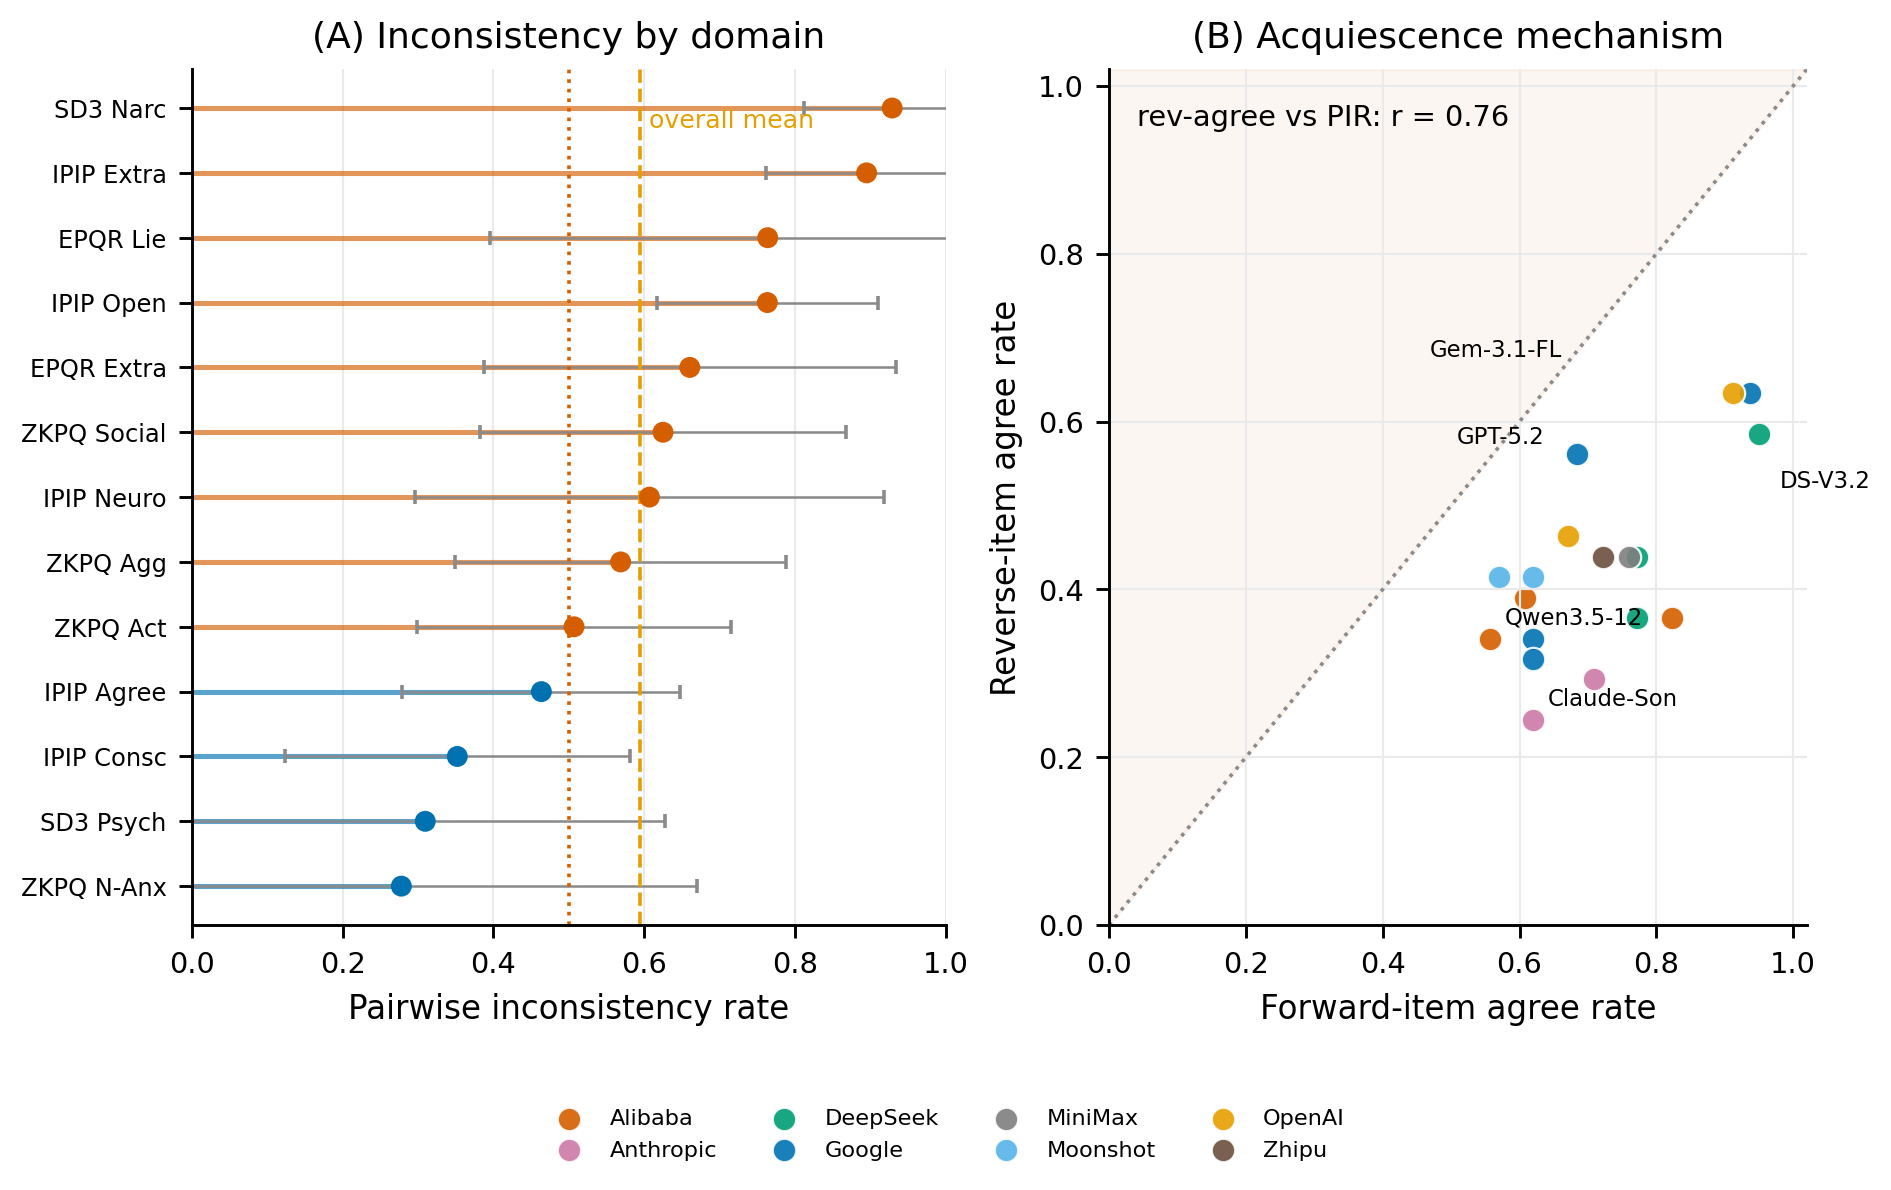
\includegraphics[width=\linewidth]{fig3_acquiescence_mechanism.png}
\caption{Reverse-item inconsistency and acquiescence mechanism. Left: PIR by domain. Right: Reverse-item agree rate vs.\ PIR ($r = 0.755$).}
\label{fig:pir_sdr_mechanism}
\end{figure}

Interestingly, persona injection \emph{improves} consistency. Under the Default prompt, PIR agreement is 0.667. Under MBTI persona prompts, it rises to 0.831 ($t = 8.96$, $p < 0.0001$). When you give a model a specific role to play, the tension between alignment-driven agreeableness and honest responding decreases. The model can be consistent within its assigned character.

\subsection{Variance Decomposition}

If these instruments are not measuring personality, what \emph{are} they measuring? \cref{tab:variance} partitions the total response variance into five sources. The answer is unambiguous: for Likert scales, \textbf{inter-model variance accounts for only 0.35\%}. Which model answered the question barely matters. What matters is which item was asked (35.2\%), which domain it belongs to (23.2\%), and residual noise (37.3\%). Binary scales tell the same story. Cross-model personality comparisons are effectively meaningless at this resolution.

\begin{table}[t]
\centering
\small
\caption{Sequential variance decomposition. Model variance: $<$1\% for both scale types.}
\label{tab:variance}
\begin{tabular}{lrr}
\toprule
Source & Likert (\%) & Binary (\%) \\
\midrule
\textbf{Model} & \textbf{0.35} & \textbf{0.47} \\
Domain & 23.21 & 5.13 \\
Persona & 3.91 & 12.93 \\
Item & 35.18 & 14.03 \\
Residual & 37.35 & 67.43 \\
\bottomrule
\end{tabular}
\end{table}

\begin{figure}[t]
\centering
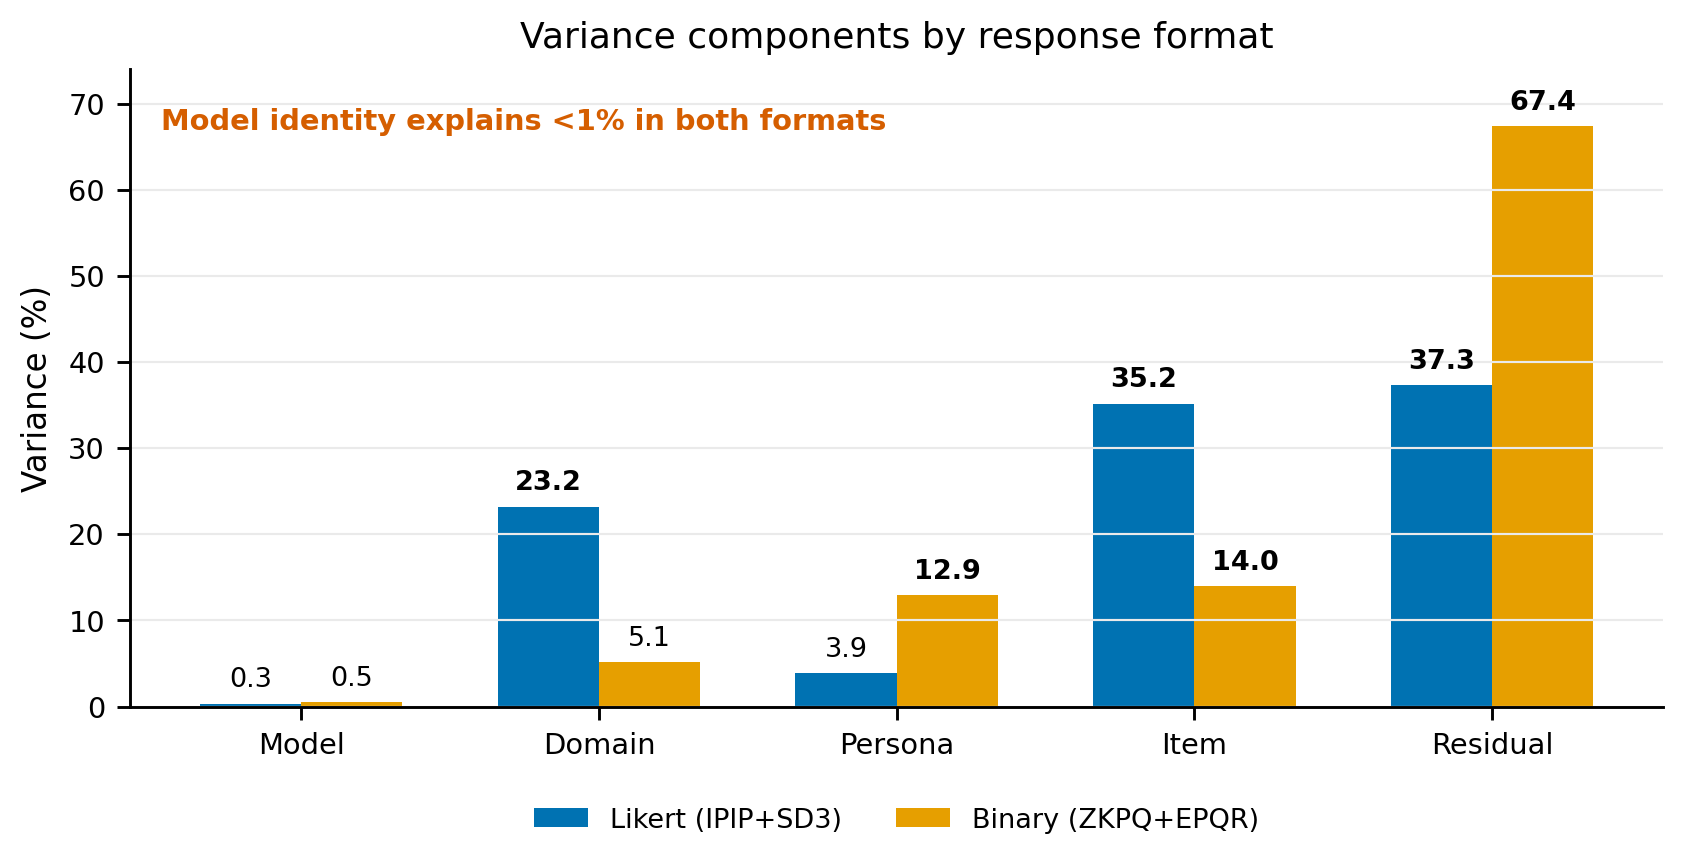
\includegraphics[width=\linewidth]{fig4_variance_decomposition.png}
\caption{Sequential variance decomposition. Inter-model variance: 0.35\% (Likert), 0.47\% (Binary).}
\label{fig:variance_decomposition}
\end{figure}

The practical implication is straightforward. If you administer a personality questionnaire to two different LLMs and get different scores, the difference is almost certainly noise, not personality.

\subsection{Convergent Validity and DIF}

One more check. If the instruments measure real traits, then related constructs across different scales should correlate in the expected direction. \cref{tab:convergent} tests 8 such pairs. Seven show the expected sign. The exception is Extraversion and Sociability, which should correlate positively but instead show a sign reversal ($r_s = -0.11$). Extraverted models in one scale are not sociable in another. The magnitudes are also weaker than human baselines across the board.

\begin{table*}[t]
\centering
\small
\caption{Convergent validity: correlations between theoretically overlapping constructs. Both Pearson ($r_p$) and Spearman ($r_s$) reported. ``OK'' = sign matches expectation.}
\label{tab:convergent}
\begin{tabular}{llrrrrc}
\toprule
Pair & Exp. & $r_p$ & $p_p$ & $r_s$ & $p_s$ & OK \\
\midrule
Neuroticism $\times$ N-Anx. & $+$ & 0.56 & 0.017 & 0.60 & 0.009 & Yes \\
Extraversion $\times$ Sociability & $+$ & $-0.03$ & 0.900 & $-0.11$ & 0.668 & \textbf{No} \\
Extraversion $\times$ Extraversion & $+$ & 0.28 & 0.254 & 0.28 & 0.261 & Yes \\
Neuroticism $\times$ Neuroticism & $+$ & 0.39 & 0.106 & 0.39 & 0.113 & Yes \\
Agreeableness $\times$ Machiavellianism & $-$ & $-0.69$ & 0.001 & $-0.71$ & 0.001 & Yes \\
Agreeableness $\times$ Psychopathy & $-$ & $-0.68$ & 0.002 & $-0.72$ & 0.001 & Yes \\
Conscientiousness $\times$ Psychopathy & $-$ & $-0.62$ & 0.006 & $-0.63$ & 0.005 & Yes \\
Psychoticism $\times$ Psychopathy & $+$ & 0.08 & 0.764 & 0.19 & 0.455 & Yes \\
\bottomrule
\end{tabular}
\end{table*}

\begin{figure}[t]
\centering
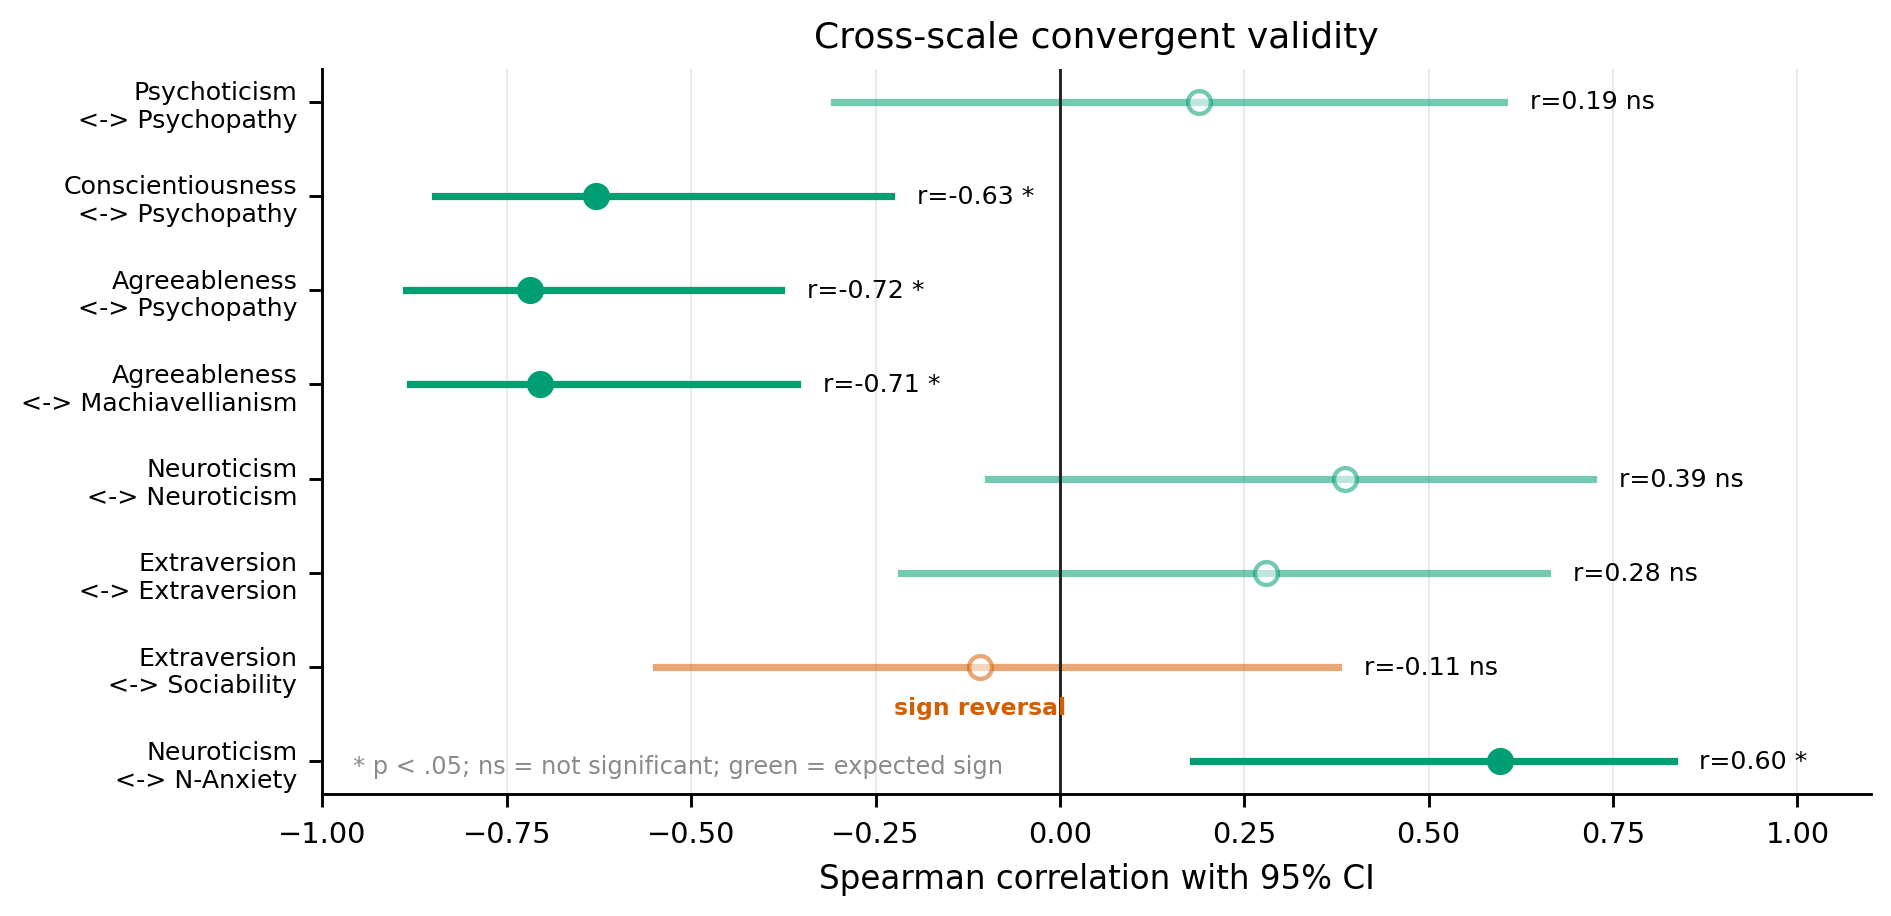
\includegraphics[width=\linewidth]{fig5_convergent_validity.png}
\caption{Convergent validity across instruments. Extraversion--Sociability shows sign reversal.}
\label{fig:convergent_validity_forest}
\end{figure}

A DIF analysis across model families found no significant differences in any domain (all $d < 0.20$; details in \cref{sec:appendix_dif}).

\subsection{Synthetic Baselines and Robustness}

\begin{table}[t]
\centering
\footnotesize
\caption{Synthetic baselines: Cronbach's $\alpha$ by domain.}
\label{tab:synthetic}
\resizebox{\columnwidth}{!}{%
\begin{tabular}{lrrrrr}
\toprule
Strategy & N & E & O & A & C \\
\midrule
Random & 0.016 & 0.042 & 0.058 & 0.077 & $-$0.026 \\
Pure Acq. & $-$0.038 & $-$0.031 & $-$0.020 & $-$0.031 & 0.005 \\
Trait+Acq. & 0.982 & 0.985 & 0.985 & 0.986 & 0.986 \\
\midrule
\textbf{LLM Obs.} & \textbf{0.749} & \textbf{0.924} & \textbf{0.193} & \textbf{0.060} & \textbf{0.517} \\
Human & 0.90 & 0.89 & 0.87 & 0.88 & 0.90 \\
\bottomrule
\end{tabular}%
}
\end{table}

\begin{figure}[t]
\centering
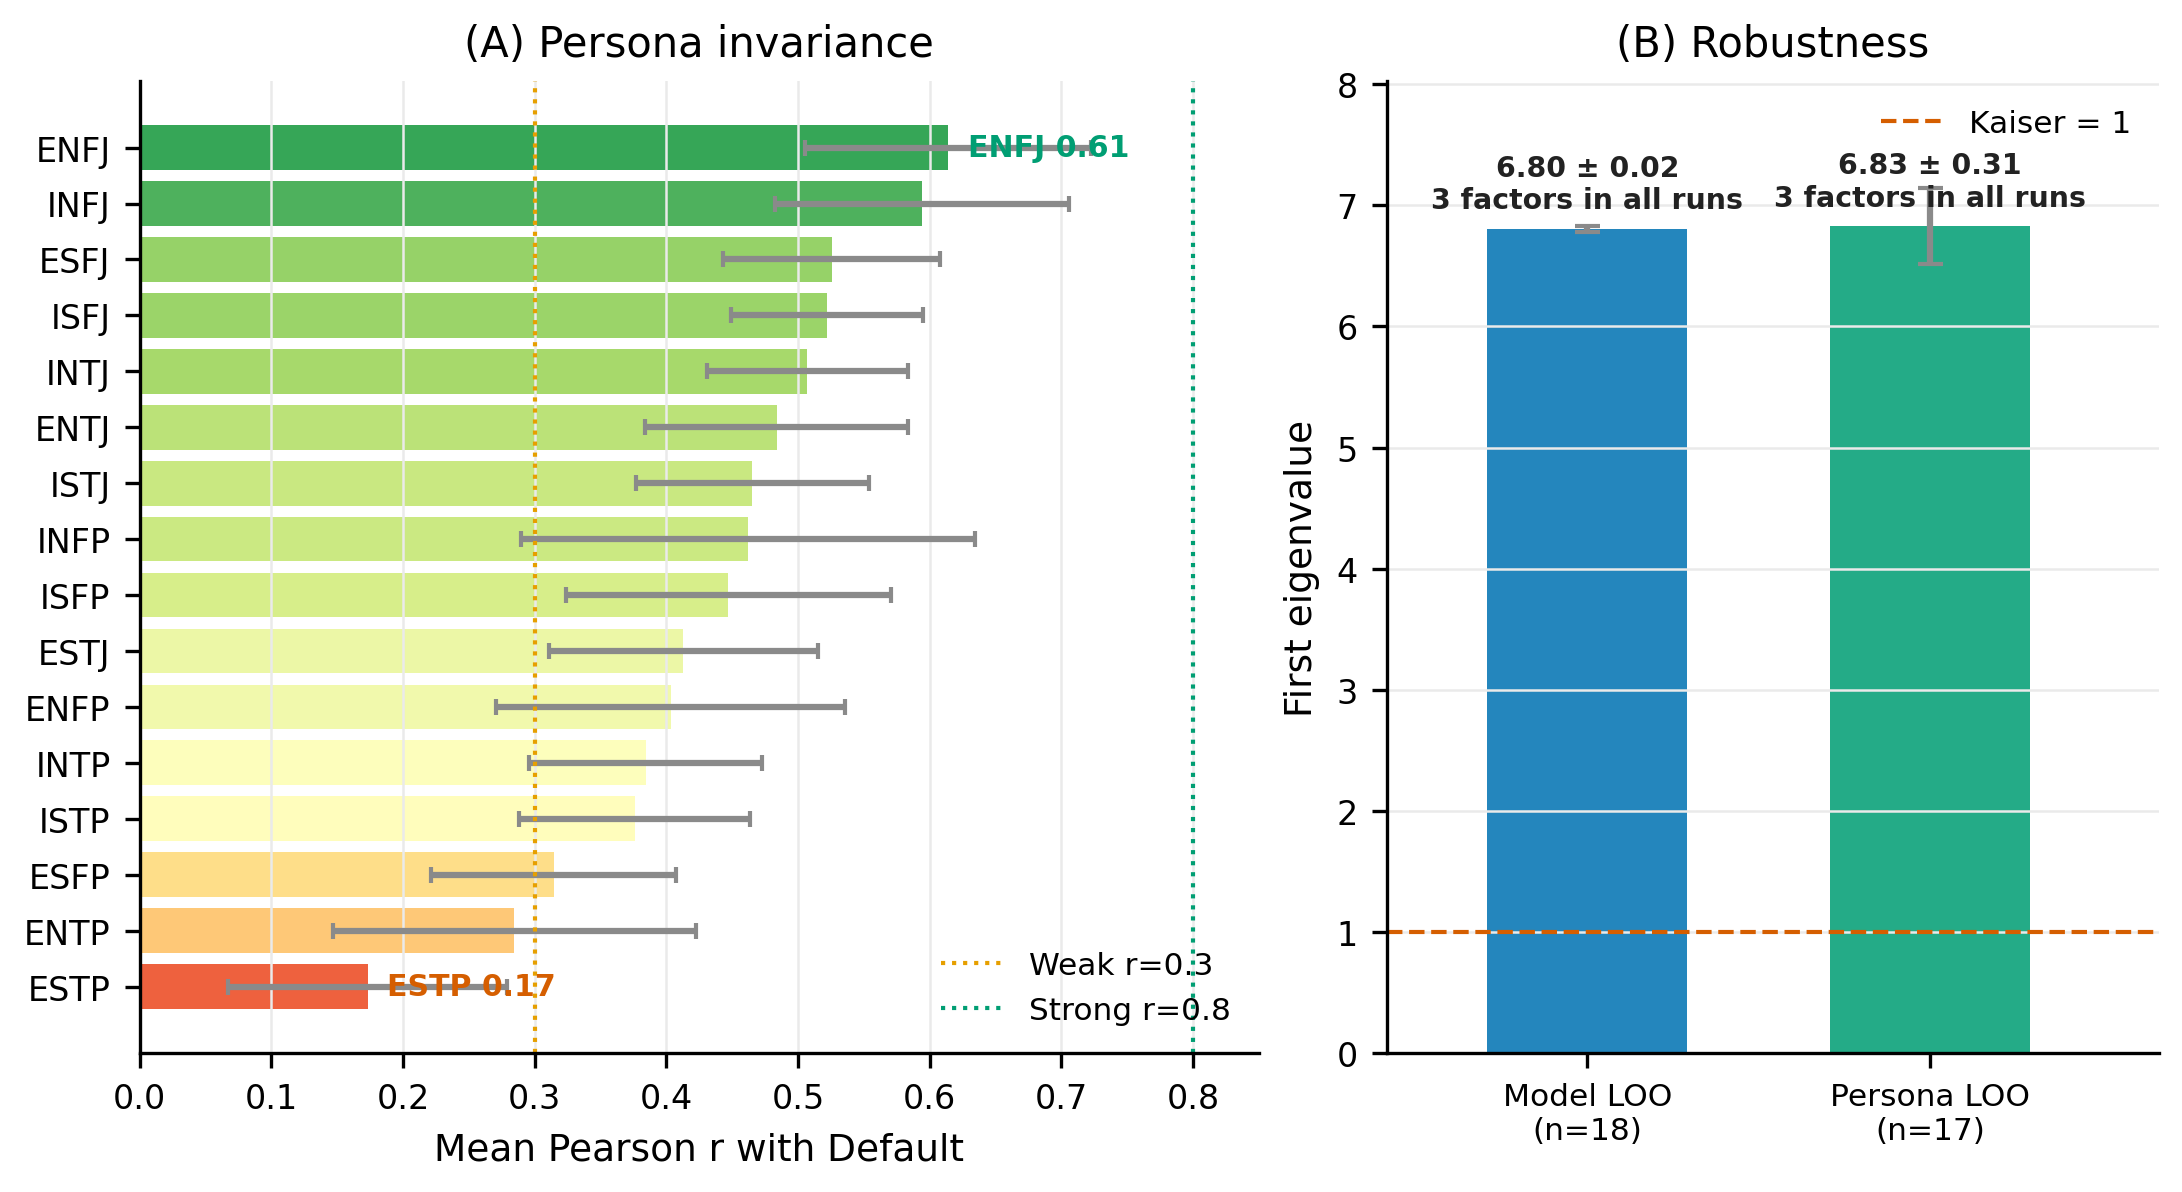
\includegraphics[width=\linewidth]{fig6_invariance_robustness.png}
\caption{Persona-level measurement invariance. Most invariant: ENFJ ($r = 0.614$). Least: ESTP ($r = 0.173$).}
\label{fig:measurement_invariance}
\end{figure}

How do LLM responses compare to simulated data? \cref{tab:synthetic} shows three baselines: random responses, pure acquiescence (always agree), and trait-plus-acquiescence (genuine structure with acquiescence). LLM alphas fall closest to the Random and Pure Acquiescence baselines. They are far from the Trait+Acquiescence strategy ($\alpha > 0.99$) that mimics genuine trait structure. In other words, LLMs do not look like they have personality with some acquiescence on top. They look like they have acquiescence with no personality underneath.

The mean Pearson correlation between Default and MBTI persona profiles is $r = 0.436$. No model-persona pair achieves strong invariance ($r > 0.8$). Changing the prompt substantially rewrites the response profile.

\subsection{Persona Prompts as a Stress Test}

The MBTI conditions act as a stress test: if the instruments measured stable traits, persona prompts should move scores without repairing the failed psychometrics. That is what we find. Persona prompts shift profiles by more than one SD from Default on average, and nearest-centroid classification recovers the prompted MBTI type in 286 of 288 cases (99.3\%). However, this is prompt compliance rather than restored validity: cross-scale persona coherence is imperfect (0.826), forward/reverse pairs move in the theoretically opposite raw-score direction only 70.4\% of the time, and the Big Five factor collapse remains. Full persona-steering analyses, including default bias, model clustering, MBTI factorial effects, scale-format sensitivity, fidelity matrices, and item plasticity, are reported in \cref{sec:appendix_persona_steering}.

\section{Conclusion}

Prior work noticed individual symptoms---inconsistent responses \citep{suhr2025challenging}, social desirability \citep{acerbi2024llm}, instability \citep{pelet2025persistent}---but treated them as separate problems. Our results show they share one root cause: acquiescence, produced by alignment training, propagating through every level of the measurement.

The evidence forms a single causal chain. At the item level, acquiescence makes LLMs agree with both forward and reverse items, so $\alpha$ tracks reverse-item density: Extraversion (17\% reverse, $\alpha = 0.92$) survives while Agreeableness (71\% reverse, $\alpha = 0.06$) collapses. At the domain level, the same bias distorts inter-domain correlations, merging Neuroticism and Agreeableness into one factor and shrinking the Big Five from five to three. At the model level, alignment training produces the same moderate-prosocial style everywhere, so inter-model variance drops below 1\%.

Two findings go beyond prior work. First, acquiescence has a directional asymmetry: for normal personality items (IPIP) models agree with forward items more than reverse (positive gap), but for dark-trait items (SD3) models \emph{reject} forward items while still agreeing with reverse ones (negative gap). Acquiescence and social desirability operate simultaneously from the same root cause. Second, the per-model correlation between reverse-item agreement and PIR ($r = 0.755$) quantifies this mechanism across 18 LLMs \citep{acquiescence2025emnlp}.

Persona injection can shift profiles by over one SD from default and is highly recoverable (99.3\% fidelity), but this does not restore measurement validity---it replaces alignment-driven acquiescence with persona-driven compliance. The scores are not measuring personality at all; they are measuring the response style that alignment training produces.

What should researchers do? Three things. First, report internal consistency, factor structure, and convergent validity before interpreting any personality score \citep{huang2024reliability, serpell2024validity, cronbach1951coefficient, binz2023psychology}. Second, establish measurement invariance before comparing across conditions. Third, use multi-temperature and multi-seed designs to separate stochastic variance from genuine trait variance. Any study that reports LLM personality profiles without these checks is likely reporting alignment artifacts, not personality.

\section{Limitations}

Our study has four main limitations. First, we use a \textbf{single administration} at temperature 0.7, preventing separation of stochastic variance from genuine trait variance. Second, we lack \textbf{base vs.\ instruct model comparisons}, so we cannot isolate alignment effects. Third, we have \textbf{no multi-seed data}. Fourth, we compare against \textbf{published human norms} rather than running human participants.

\section*{Ethics Statement}

This study uses publicly available LLMs and public-domain psychometric instruments. No human subjects were involved. We do not claim that LLMs have or lack genuine personality; our contribution concerns the \emph{measurement properties} of the instruments when applied to a novel population.

\bibliographystyle{acl_natbib}
\bibliography{refs}

\clearpage
\appendix

\section{Persona Steering Supplement}
\label{sec:appendix_persona_steering}

All persona-steering diagnostics are computed from the same 67{,}626 completed item responses. These analyses are not the primary evidence for the paper's central claim. Instead, they answer a complementary question: once we know the instruments fail standard psychometric checks, what exactly happens when we deliberately push the model with a persona prompt? The answer is consistent across the analyses below. Persona prompts produce large, highly recoverable role-playing shifts, but those shifts do not repair the instrument: factor structure, reverse-item behavior, and cross-scale coherence remain contaminated by response style.

The full numerical outputs are provided as machine-readable tables: \texttt{default\_bias\_index.csv}, \texttt{persona\_target\_adherence.csv}, \texttt{persona\_fidelity\_confusion.csv}, \texttt{persona\_fidelity\_detail.csv}, \texttt{cross\_scale\_persona\_coherence.csv}, \texttt{factorial\_mbti\_effects.csv}, \texttt{item\_plasticity.csv}, and \texttt{directional\_pair\_coherence.csv}. These tables contain the complete 16$\times$16 confusion matrix, per-model persona adherence scores, item-level plasticity ranks, and distance-metric ablations.

\subsection{Model Family and Persona Effects}

This section asks whether model identity or persona instructions dominate the auxiliary structure. The first check is model clustering under the Default prompt. If LLMs had stable model-specific personality profiles, we would expect vendor or family clusters to appear in the 17-domain profile space. Instead, model-family clustering is weak. Ward-linkage clustering on z-scored Default profiles does not recover vendor groups cleanly: DeepSeek-V4-Flash clusters with Qwen3-235B, while Claude models cluster with DeepSeek-V3.2/V4-Pro. Cross-family distance is only 1.27$\times$ within-family distance. This supports the main-text variance decomposition: differences between model families are small compared with shared alignment-shaped response tendencies.

\begin{figure}[t]
\centering

\includegraphics[width=\linewidth]{fig7_model_clustering.png}
\caption{Hierarchical clustering of 18 models by z-scored Default domain profiles. Models do not cluster cleanly by vendor.}
\label{fig:clustering}
\end{figure}

The second check asks whether MBTI prompts are interpreted compositionally. They are. \cref{fig:mbti_effects} shows that the E/I axis dominates social and energetic traits: E/I has the largest effects on EPQR Extraversion ($\beta=1.01$), ZKPQ Sociability ($\beta=0.98$), IPIP Extraversion ($\beta=0.96$), SD3 Narcissism ($\beta=0.94$), and ZKPQ Activity ($\beta=0.87$). J/P mainly affects IPIP Conscientiousness ($\beta=0.96$), ZKPQ Impulsive Sensation Seeking ($\beta=-0.81$), EPQR Lie ($\beta=0.78$), and EPQR Psychoticism ($\beta=-0.73$). S/N primarily affects IPIP Openness ($\beta=0.77$), while T/F strongly affects IPIP Agreeableness ($\beta=0.93$), EPQR Neuroticism ($\beta=0.87$), and SD3 Machiavellianism ($\beta=-0.76$).

This is important because it rules out a trivial failure mode. The persona prompts are not ignored. Models do read and operationalize the MBTI instruction. However, successful role uptake is not the same thing as valid personality measurement. The role effects are large and stereotype-consistent, but the main psychometric failures remain: the Big Five still collapses, model variance remains tiny, and reverse-coded items remain contaminated.

\begin{figure}[t]
\centering
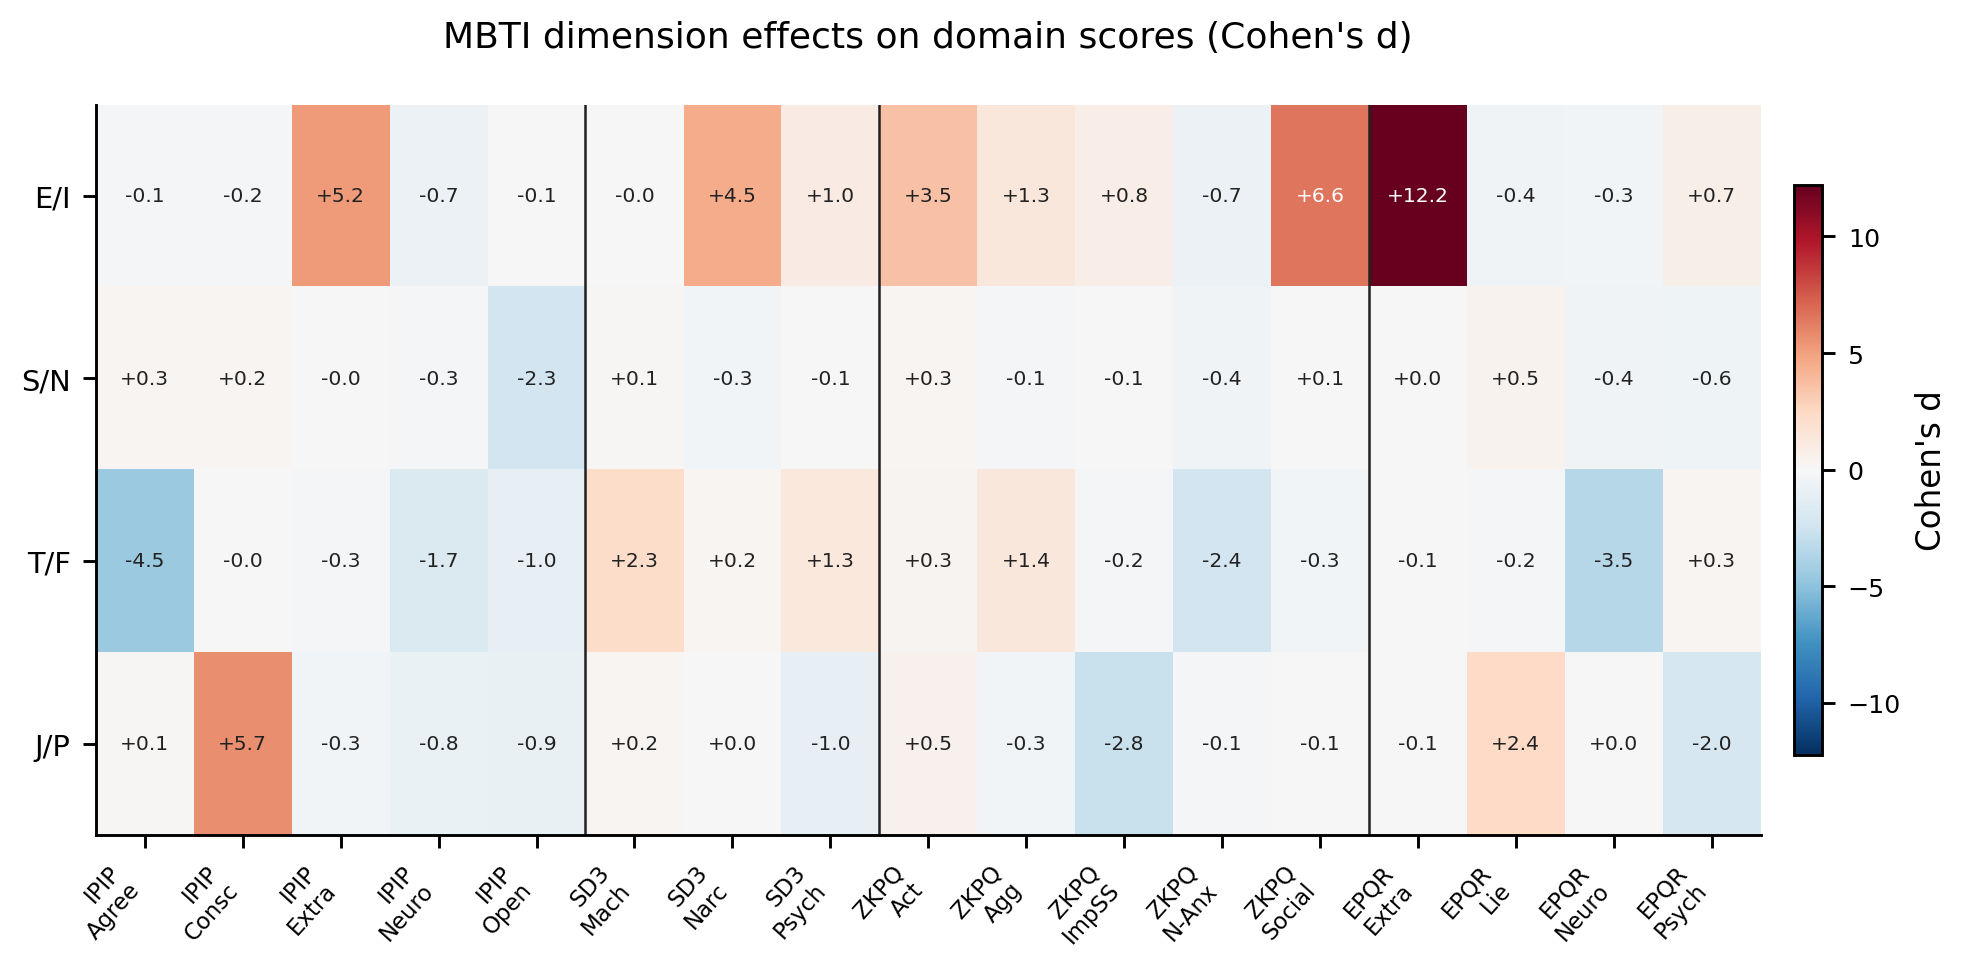
\includegraphics[width=\linewidth]{fig8_mbti_dimension_effects.png}
\caption{Cohen's $d$ effect sizes for each MBTI dimension on domain scores.}
\label{fig:mbti_effects}
\end{figure}

Scale format also matters. Binary-format scales are 75\% more sensitive to persona injection than Likert scales after normalizing by scale range. This is a methodological warning: forced yes/no formats amplify persona-induced movement, but amplification is not necessarily higher validity. In our classification ablation below, binary-only profiles are less stable than Likert or IPIP-only profiles. The binary scales therefore make prompt effects easier to see, while also reducing graded trait information.

\begin{figure}[t]
\centering

\includegraphics[width=\linewidth]{fig9_persona_sensitivity.png}
\caption{Persona sensitivity by scale format. Binary scales show larger normalized shifts.}
\label{fig:persona_sensitivity}
\end{figure}

\subsection{Persona Separation and Fidelity}

The previous section showed that MBTI prompts produce interpretable main effects. We next ask two stricter questions. First, how far does each persona move a model from its own Default baseline? Second, does the movement go toward the requested persona, or merely perturb the response profile?

\begin{table}[t]
\centering
\small
\caption{Persona Separation Degree by model. $\overline{\mathrm{PSD}}$: mean across 16 personas. $\mathrm{PSD}_{\max}$: peak. CV: coefficient of variation.}
\label{tab:psd}
\resizebox{\columnwidth}{!}{%
\begin{tabular}{lrrrr}
\toprule
Model & $\overline{\mathrm{PSD}}$ & $\mathrm{PSD}_{\max}$ & CV & Peak persona \\
\midrule
\multicolumn{5}{l}{\textit{Top 5 (most malleable)}} \\
Gemini-3-Pro & 1.425 & 2.14 & 0.229 & ENTP \\
Gemini-3.1-Pro & 1.363 & 2.07 & 0.239 & ENTP \\
Qwen3-235B & 1.356 & 1.74 & 0.172 & ESTJ \\
Gemini-3.1-Flash & 1.278 & 1.47 & 0.127 & ESTP \\
Gemini-3-Flash & 1.275 & 1.79 & 0.245 & ENTP \\
\multicolumn{5}{l}{\textit{Bottom 5 (least malleable)}} \\
Claude-Sonnet-4.6 & 1.121 & 1.72 & 0.261 & ESTP \\
DeepSeek-V3.2 & 1.111 & 1.40 & 0.191 & ENTP \\
DeepSeek-V4-Pro & 1.104 & 1.38 & 0.178 & ESTJ \\
GPT-5.5 & 1.133 & 1.53 & 0.210 & ESTP \\
MiniMax-M2.7 & 1.033 & 1.41 & 0.241 & INFP \\
\midrule
\textbf{Mean (all 18)} & \textbf{1.201} & \textbf{1.69} & \textbf{0.204} & \\
\bottomrule
\end{tabular}%
}
\end{table}

Persona Separation Degree (PSD) answers the first question by measuring the normalized Euclidean distance between a persona profile and the same model's Default profile in the 17-domain z-scored space. All models can be shifted: even MiniMax-M2.7, the least malleable model, averages $\overline{\mathrm{PSD}} = 1.03$. The most malleable model, Gemini-3-Pro, averages $\overline{\mathrm{PSD}} = 1.43$. Thus, persona prompting is not a subtle perturbation; it shifts each domain by roughly one standard deviation on average. Extraverted-Perceiving personas (ESTP, ENTP) trigger the most separation, while Introverted-Judging personas trigger the least. This asymmetry is consistent with the main-effect analysis: E/P prompts push activity, sociability, impulsivity, and narcissism away from the aligned Default profile.

Default profiles are not neutral. By nearest leave-one-model-out persona centroid, 6 of 18 Default profiles are closest to ISTJ, followed by ISTP (4/18), INTP (3/18), ISFP (2/18), INTJ (2/18), and INFP (1/18). By empirical MBTI-axis projection, 9 of 18 models are classified as ISTJ-like under Default. This means that ``no persona'' is not an empty baseline. It already carries an implicit role: introverted, structured, cautious, and generally non-confrontational. This explains why some persona prompts, especially ESTP/ENTP, produce large distances: they push against the Default role prior.

Target adherence answers the second question. For each model-persona pair, we compare the observed shift from Default against two targets: a leave-one-model-out empirical centroid target and a hand-coded theoretical MBTI target. Persona-conditioned shifts align strongly with the empirical target (mean cosine 0.816 [0.774, 0.856]) but less strongly with the theory-only target (0.547). The strongest empirical adherence appears for ESTP (0.901), ENTP (0.890), and ENFP (0.888); the weakest appears for INTP (0.699), ISTP (0.714), and INTJ (0.739). At the model level, Qwen3.5-397B, Kimi-K2.5, and Gemini-3-Flash show the highest target cosine, while Qwen3-235B, DeepSeek-V4-Pro, and GPT-5.2 are lowest. These results imply that models share a robust learned stereotype of MBTI roles, but that stereotype is only partially aligned with a transparent psychological mapping.

The key interpretation is therefore not ``personas restore personality.'' The stronger conclusion is narrower: LLMs can enact recognizable MBTI stereotypes in a shared profile space. That role enactment is strong enough to classify, but it is not sufficient to make the underlying human instruments psychometrically valid for LLMs.

\begin{figure*}[t]
\centering
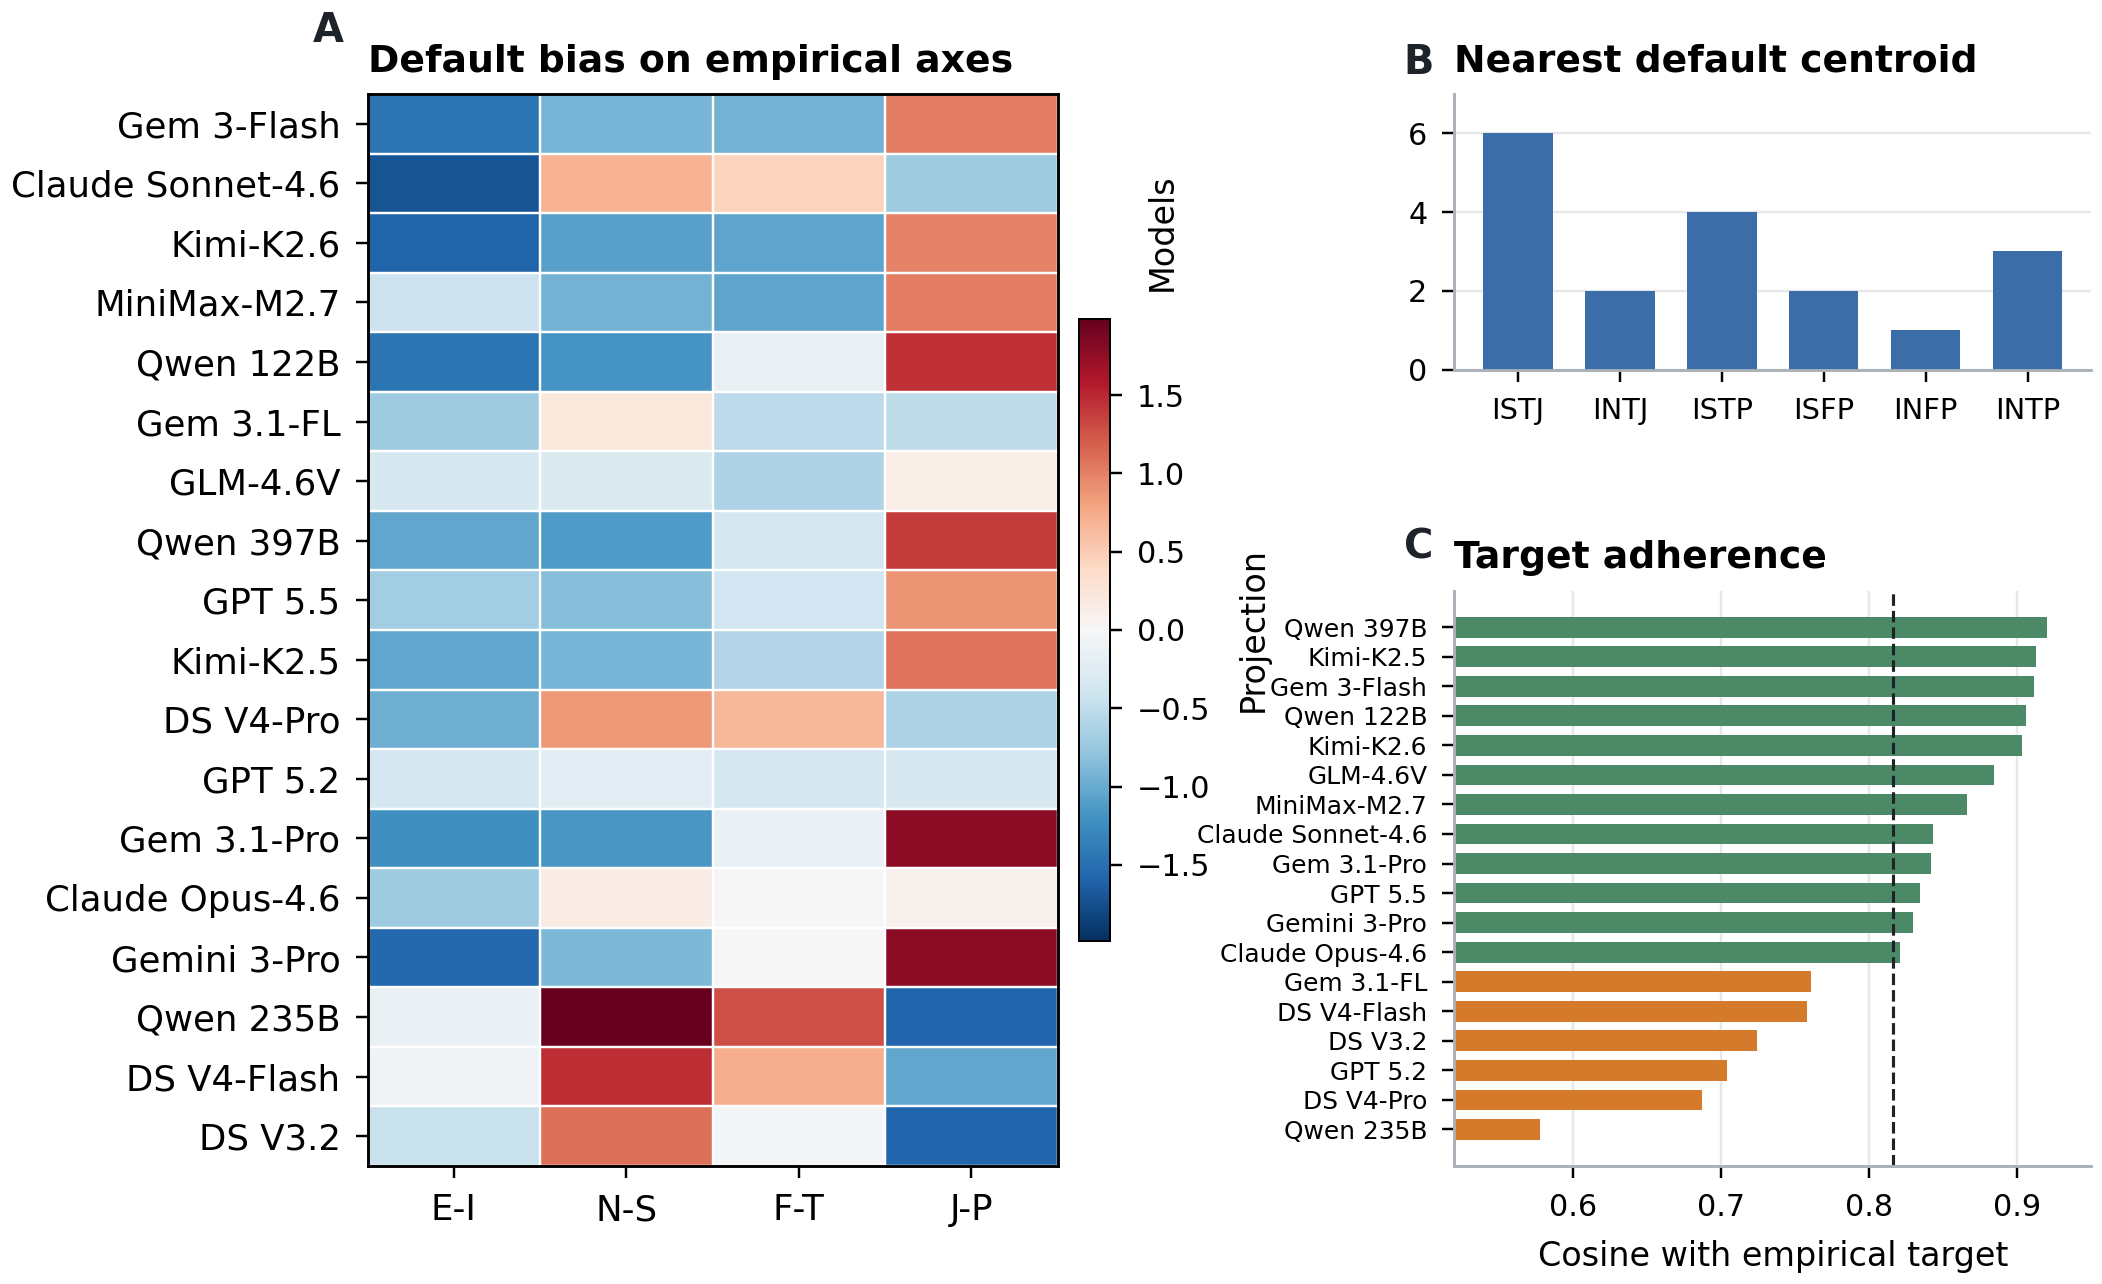
\includegraphics[width=\linewidth]{fig11_default_bias_and_adherence.png}
\caption{Default bias and persona target adherence.}
\label{fig:default_bias_adherence}
\end{figure*}

Persona-conditioned profiles are highly classifiable: nearest-centroid classification recovers 286/288 prompted MBTI types (99.3\%). The two confusions are Claude-Opus-4.6 ISFJ $\rightarrow$ INFJ and DeepSeek-V3.2 ESTJ $\rightarrow$ ENTJ, both with very small margins (0.010 and 0.019 in normalized distance). This is the strongest evidence that the prompt manipulation itself worked. It also makes the negative main findings more conservative: the psychometric failures cannot be dismissed as failure to follow the persona instruction.

The result is robust to distance metric and scale subset. Accuracy is 98.6\% under cosine distance and 96.2\% under Mahalanobis distance. Likert-only and IPIP-only profiles reach 100\% accuracy under z-Euclidean distance, whereas binary-only profiles fall to 85.8\%. This supports two conclusions. First, the persona signal is strongest in graded Likert/IPIP responses. Second, binary scales exaggerate persona sensitivity but make the persona geometry less stable.

\begin{figure}[t]
\centering
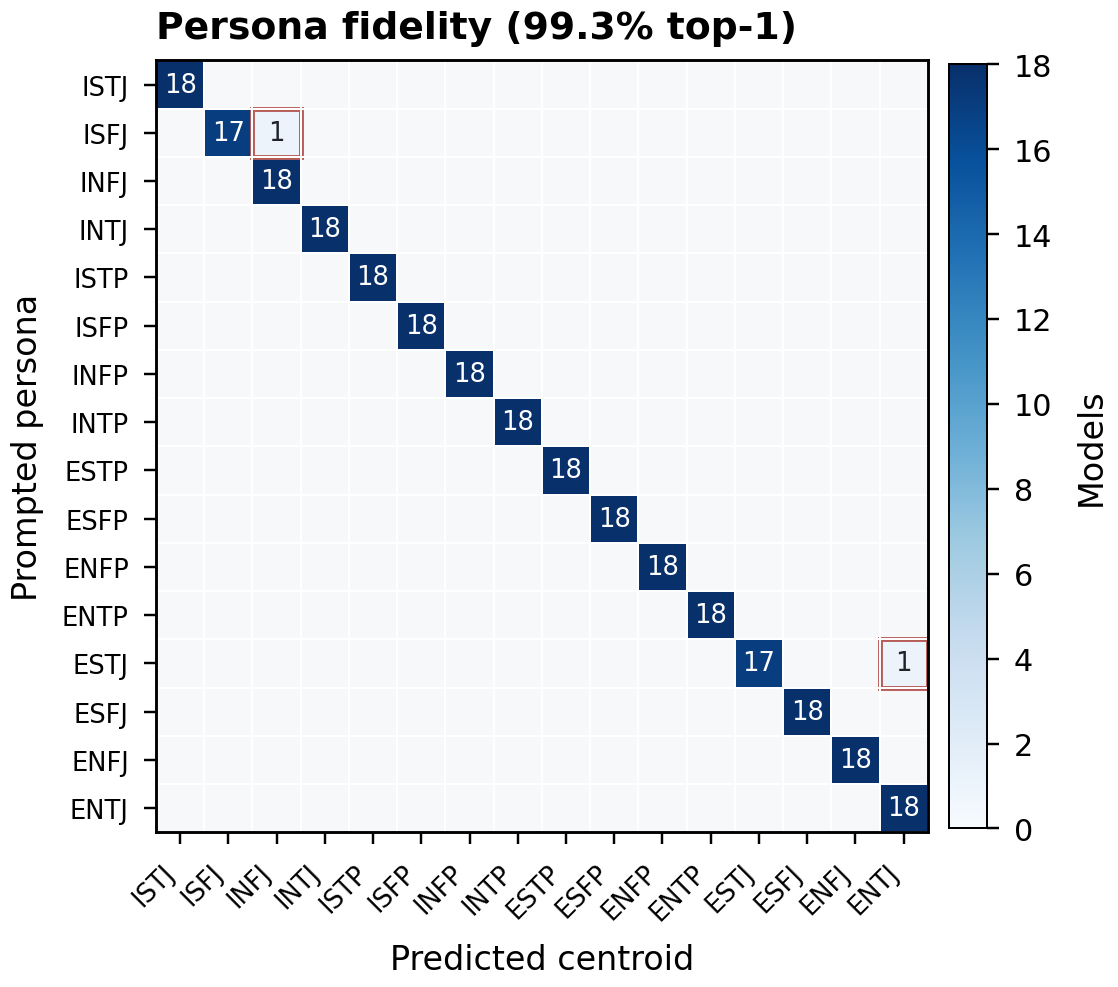
\includegraphics[width=\linewidth]{fig12_persona_fidelity_confusion.png}
\caption{Persona fidelity confusion matrix using leave-one-model-out centroids.}
\label{fig:persona_confusion}
\end{figure}

\begin{figure}[t]
\centering
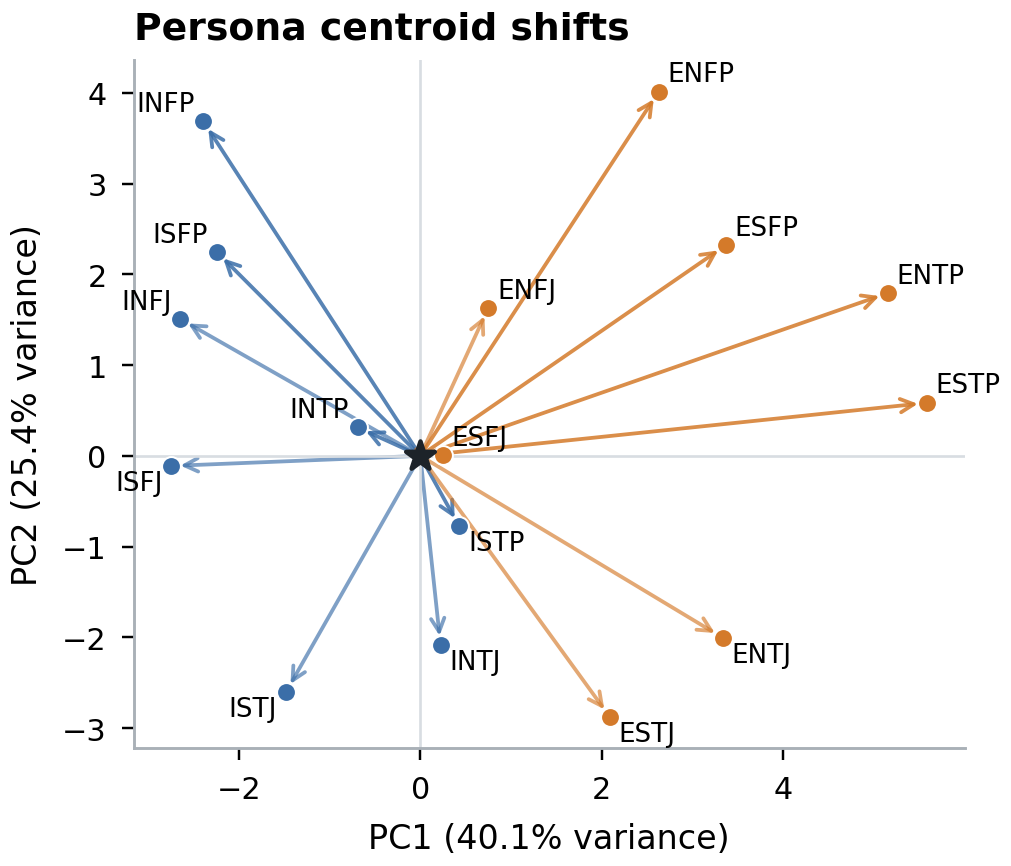
\includegraphics[width=\linewidth]{fig14_persona_vector_field.png}
\caption{Persona centroid shifts from Default in the first two principal components of 17-domain profile space.}
\label{fig:persona_vector_field}
\end{figure}

\subsection{Cross-scale Coherence and Item Plasticity}

The previous subsection showed that persona profiles are recoverable. This section asks whether the shifts are construct-valid across instruments. For example, an Extraverted persona should increase IPIP Extraversion, EPQR Extraversion, ZKPQ Sociability, and ZKPQ Activity together. A Feeling persona should increase Agreeableness while decreasing antagonistic traits such as Machiavellianism, Psychopathy, and Aggression-Hostility. We therefore sign-align overlapping constructs and compute a coherence score: 1 means all scales move in the same construct direction, while 0 means the movement cancels across scales.

Overlapping constructs move together, but unevenly. Mean cross-scale coherence is 0.826 [0.801, 0.851], with a sign-match rate of 0.775. Extraversion is most coherent (0.882; sign-match 0.867), followed by Neuroticism (0.850; sign-match 0.746). Agreeableness versus antagonism (0.784) and Conscientiousness versus disinhibition (0.790) are weaker. The lower coherence for moralized and impulse-control constructs is theoretically important: these are the same regions where alignment and safety constraints are strongest, so persona role-play has less freedom to move all instruments consistently.

The persona-level pattern reinforces this interpretation. ESTP and ENTP show the highest average coherence (0.962 and 0.948), because they strongly activate the same extraversion/activity/disinhibition dimensions across scales. INTJ and ISTJ show the lowest coherence (0.701 and 0.729), because their shifts are smaller and more constrained. Thus, coherence is highest when the persona prompt pushes models along broad behavioral dimensions and weakest when the prompt asks for restrained, low-variance profiles close to Default.

\begin{figure*}[t]
\centering
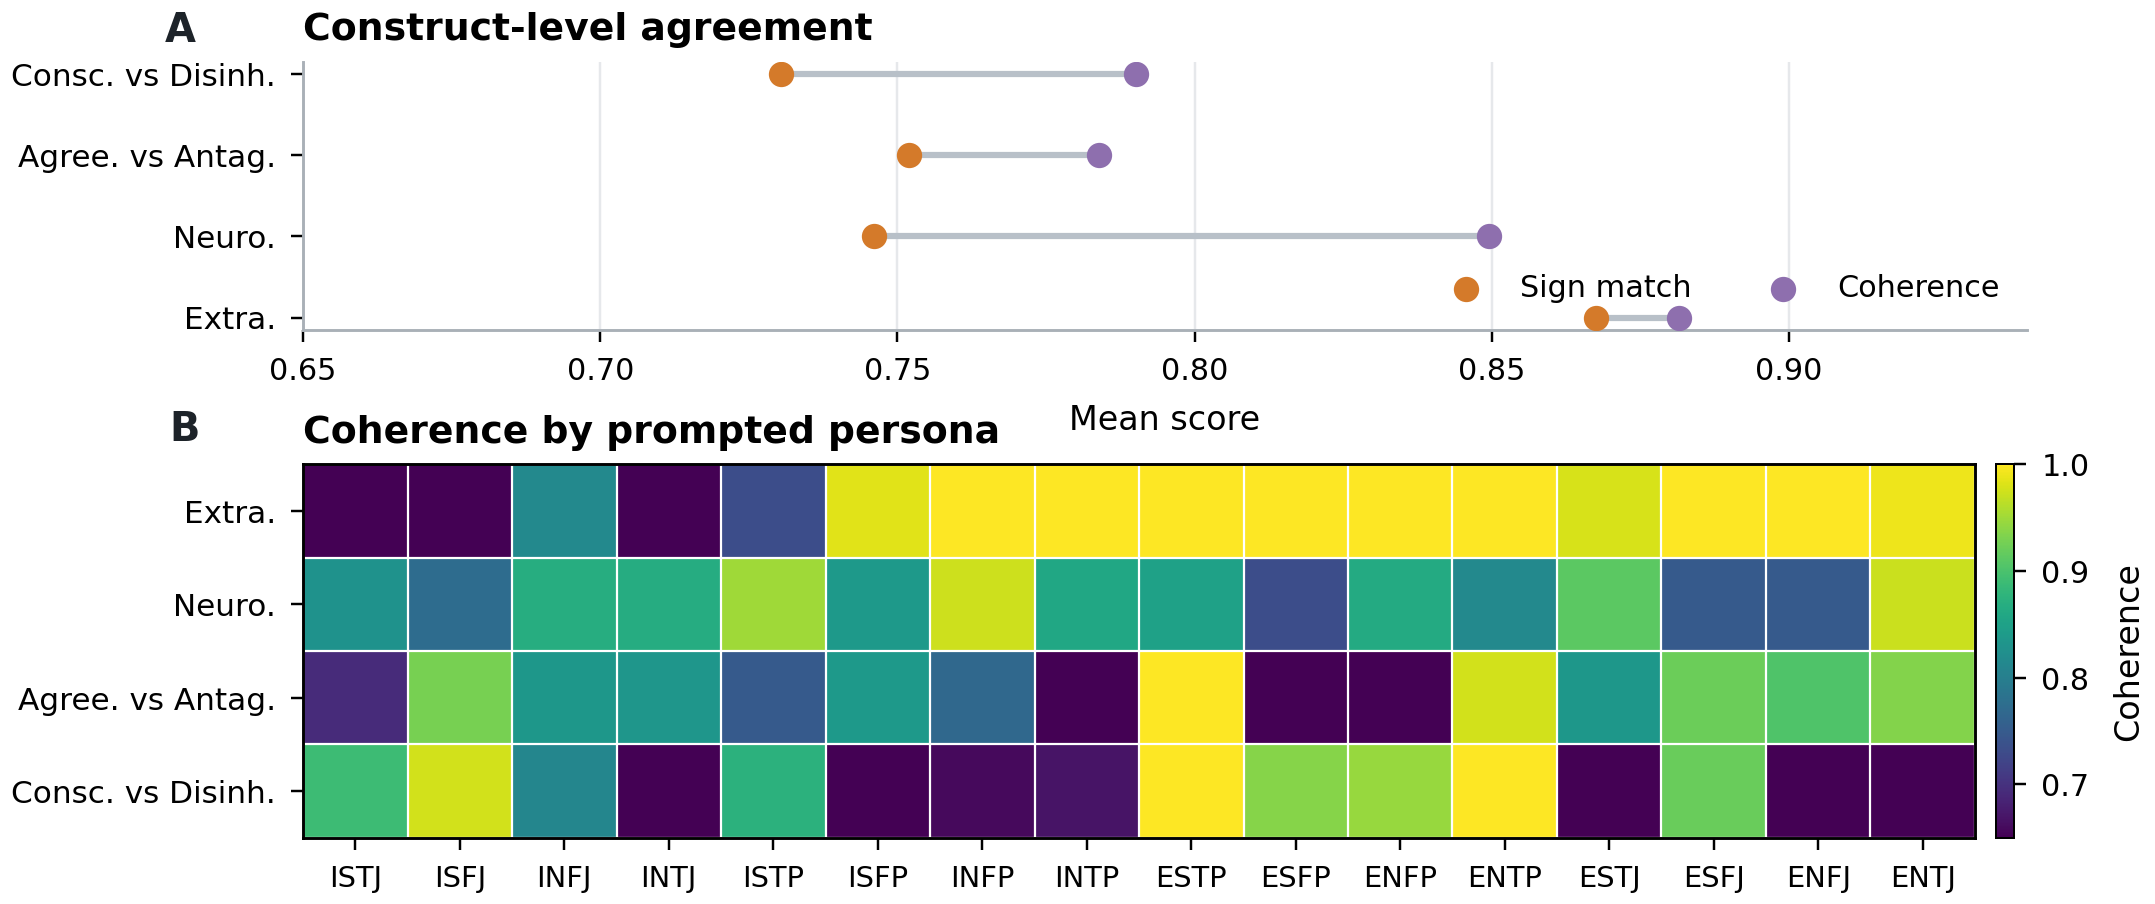
\includegraphics[width=\linewidth]{fig13_cross_scale_persona_coherence.png}
\caption{Cross-scale persona coherence.}
\label{fig:cross_scale_persona_coherence}
\end{figure*}

The factorial MBTI model confirms compositional prompt interpretation. The largest effects are E/I on EPQR Extraversion ($\beta=1.01$), ZKPQ Sociability ($\beta=0.98$), IPIP Extraversion ($\beta=0.96$), and SD3 Narcissism ($\beta=0.94$); J/P on IPIP Conscientiousness ($\beta=0.96$); S/N on Openness ($\beta=0.77$); and T/F on Agreeableness ($\beta=0.93$). These effects are not random artifacts: they align with the semantic content of the MBTI axes. However, the same model also reveals leakage. EPQR Lie loads strongly on J/P ($\beta=0.78$), and SD3 Narcissism loads strongly on E/I. This means persona prompts alter response style and self-presentation, not only target traits.

Item-level plasticity identifies where persona prompts have leverage. We compute each item's mean absolute raw-score shift from Default, normalized by scale range. The most plastic items are activity, sociability, and rule-following items: ``Do you sometimes talk about things you know nothing about?'' (0.632), ``I lead a busier life than most people'' (0.608), ``Do you prefer to go your own way rather than act by the rules?'' (0.597), and activity/sociability items from ZKPQ. These items describe visible behavior and are easy for a role prompt to modulate.

The most locked items are different. They include ``Do you enjoy hurting people you love?'' (0.000), ``Are all your habits good and desirable ones?'' (0.010), ``Do you enjoy practical jokes that can sometimes really hurt people?'' (0.031), ``Take advantage of others'' (0.056), and ``Insult people'' (0.075). Many are safety-sensitive, moralized, or socially undesirable. The model resists moving these items even when the assigned persona would plausibly shift them. This is direct item-level evidence for the alignment constraint proposed in the main text: persona instructions can move ordinary behavioral descriptors, but they do not freely override safety- and desirability-shaped response patterns.

Finally, forward/reverse pairs move in the theoretically opposite raw-score direction only 70.4\% of the time. By scale, directional pair coherence is highest for EPQR-A (0.784) and ZKPQ-50-CC (0.748), lower for SD3 (0.693), and lowest for IPIP-NEO-120 (0.679). This residual failure is why persona steering does not rescue the measurement. The model can adopt a role well enough to classify the prompt, yet still fail the forward/reverse logic that validated human personality scales depend on.

\begin{figure*}[t]
\centering
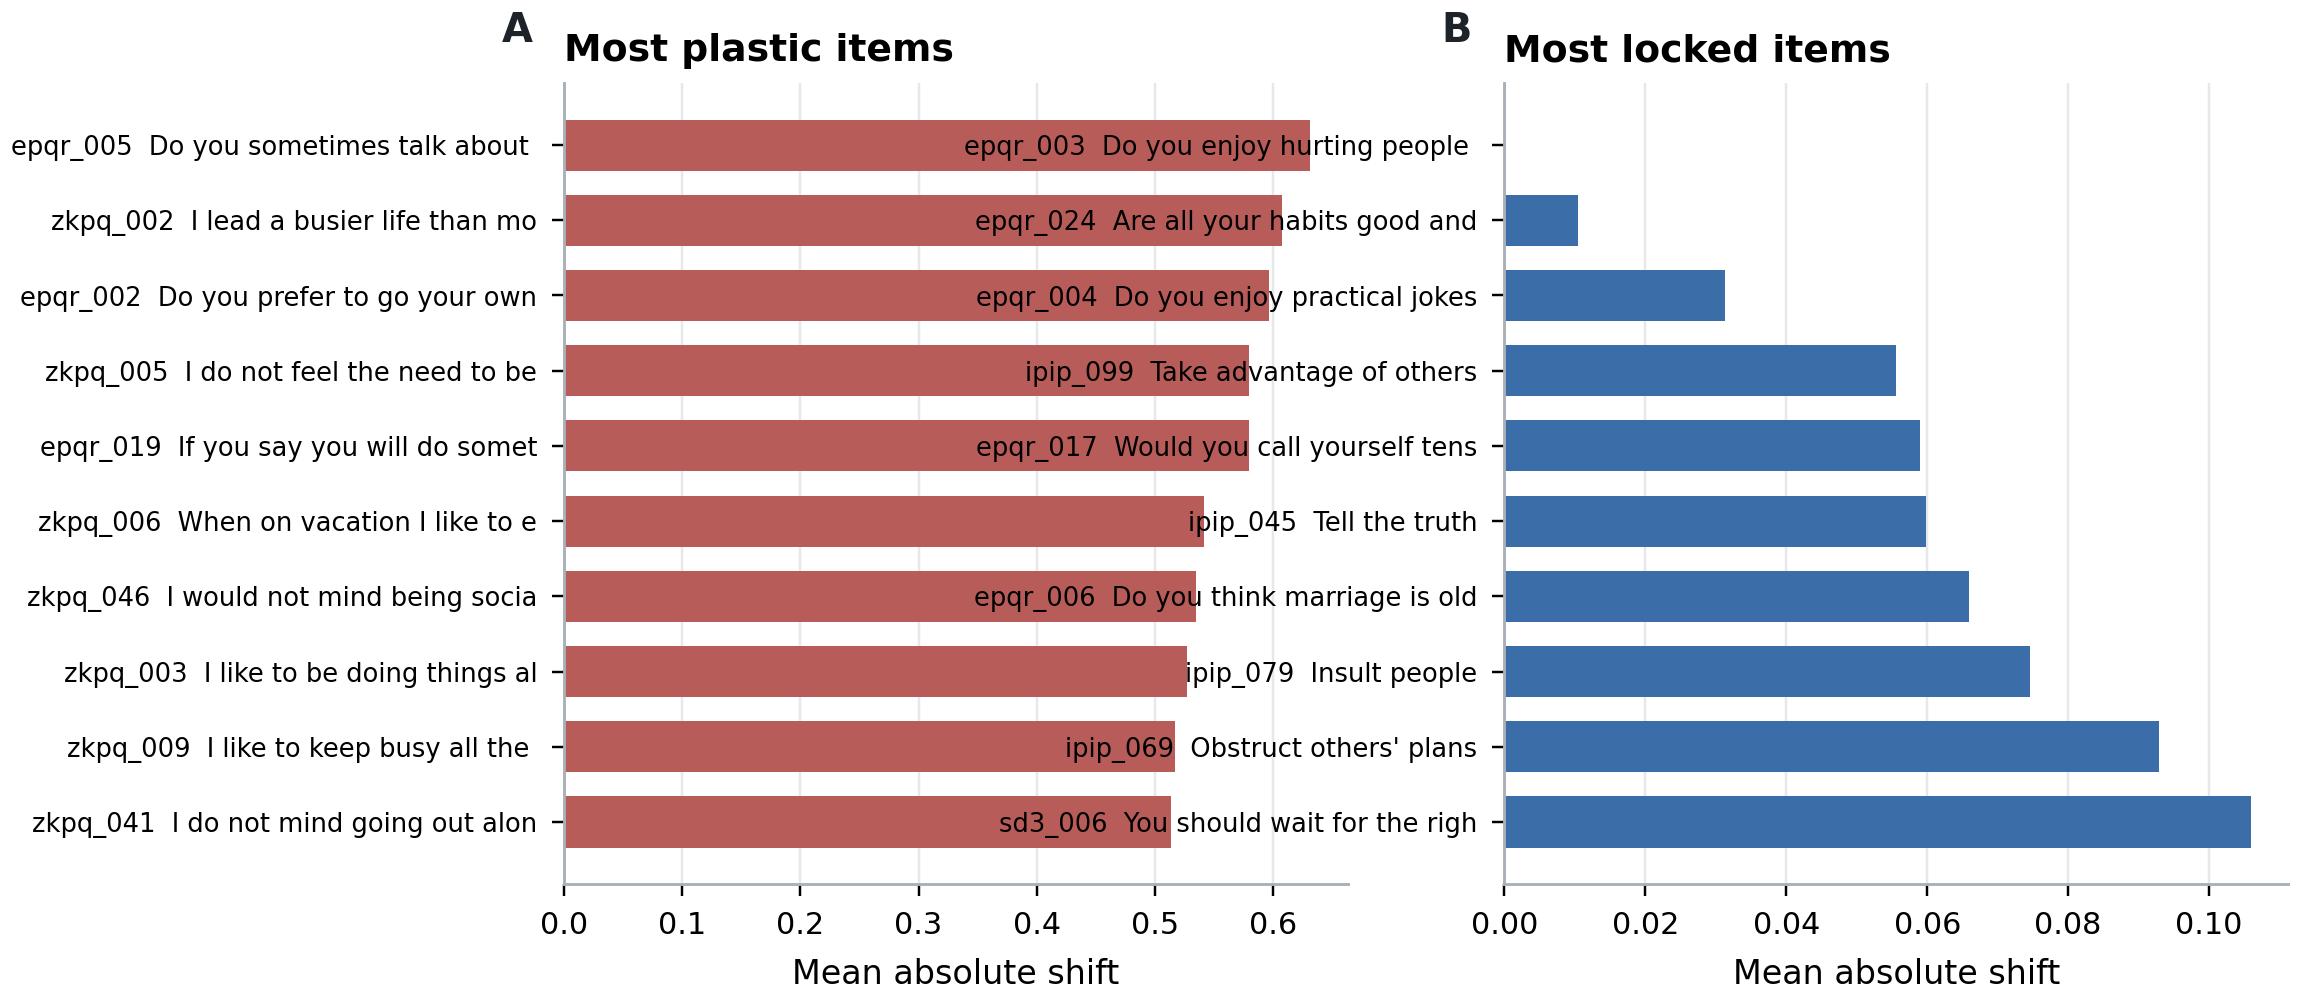
\includegraphics[width=\linewidth]{figA1_item_plasticity.png}
\caption{Most plastic and most locked items under MBTI persona steering. Plastic items are mostly activity, sociability, and rule-following items; locked items are concentrated in safety- and morality-sensitive content.}
\label{fig:appendix_item_plasticity}
\end{figure*}

\begin{figure}[t]
\centering
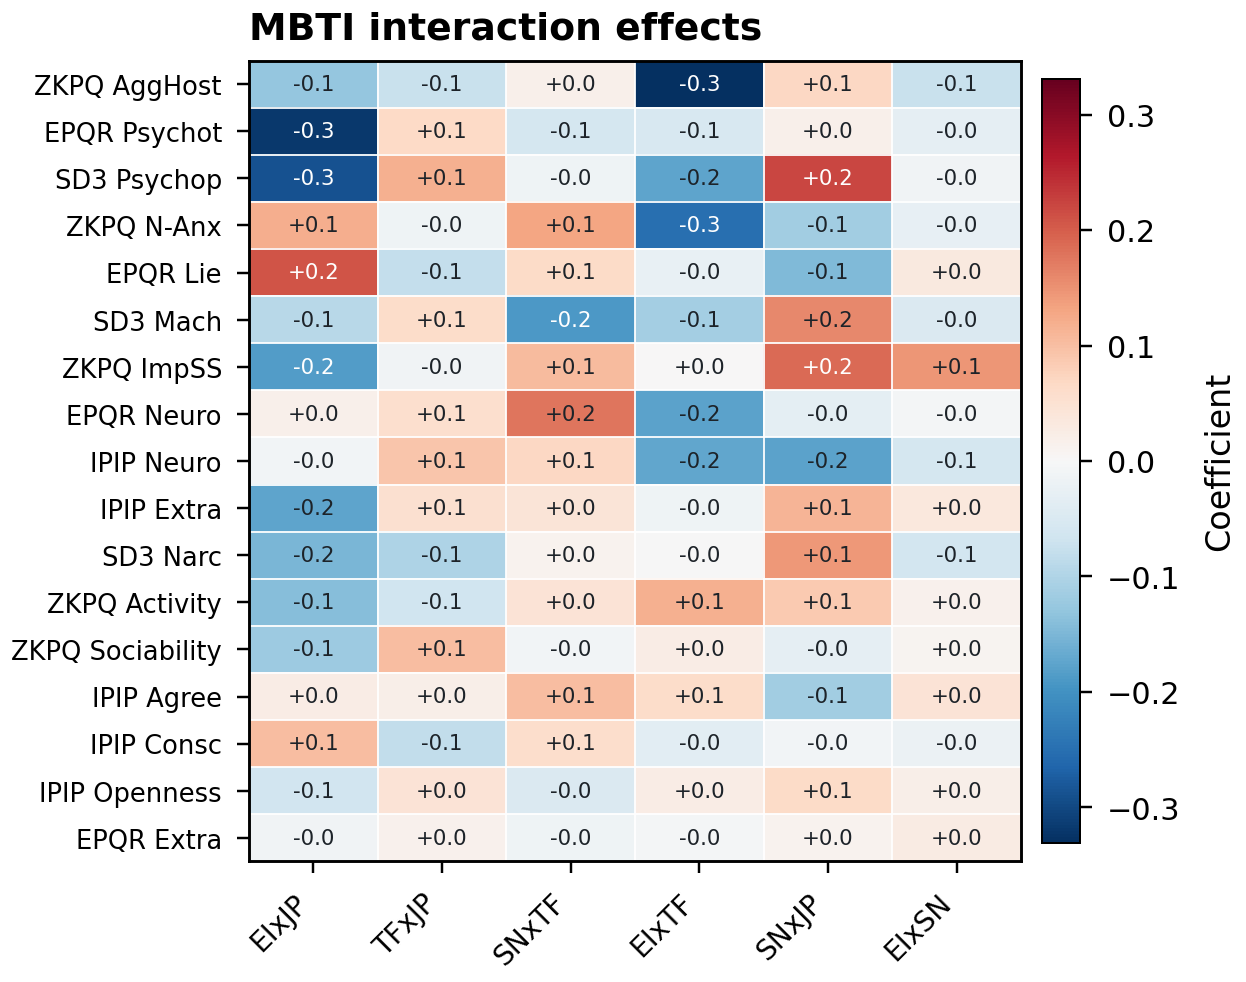
\includegraphics[width=\linewidth]{figA2_mbti_interactions.png}
\caption{Two-way MBTI interaction coefficients from the factorial model. Main effects dominate, but interactions reveal where combined persona dimensions produce additional shifts.}
\label{fig:appendix_mbti_interactions}
\end{figure}

\begin{figure}[t]
\centering
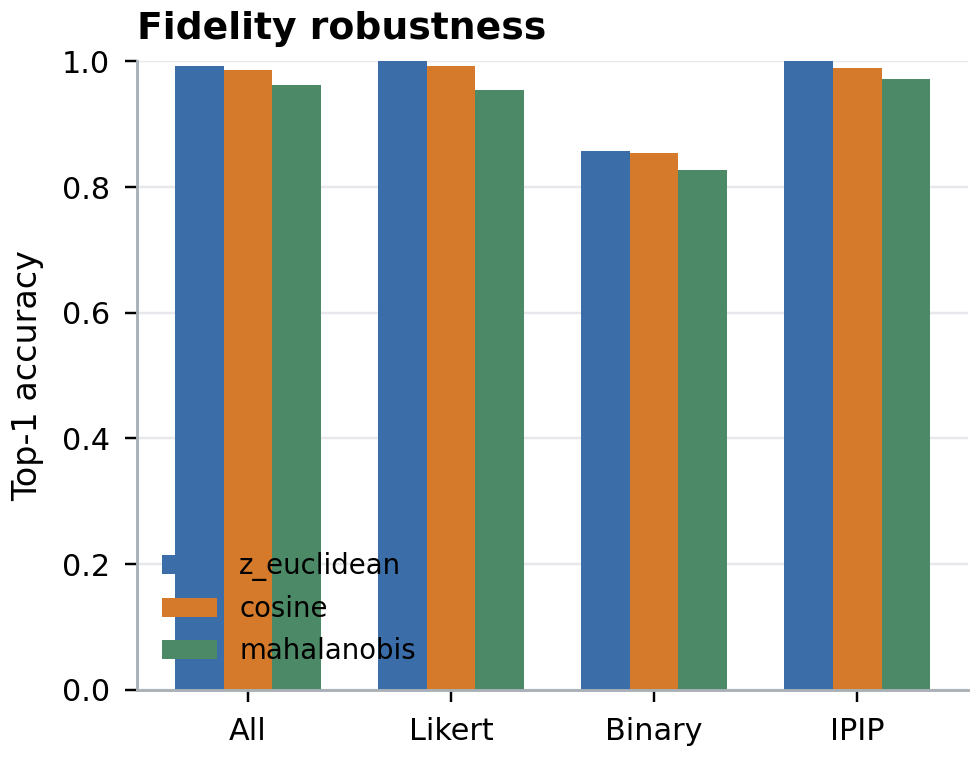
\includegraphics[width=\linewidth]{figA3_robustness_sensitivity.png}
\caption{Persona-fidelity robustness across distance metrics and scale ablations. Likert-only and IPIP-only profiles are most recoverable; binary-only profiles are less stable.}
\label{fig:appendix_robustness}
\end{figure}

\section{DIF Across Model Families}
\label{sec:appendix_dif}

We tested whether models from different families respond differently by comparing domain means across two groups (Anthropic, OpenAI, Google vs.\ DeepSeek, Alibaba, Moonshot, MiniMax, Zhipu). No domain showed a significant difference (\cref{tab:dif_appendix}).

\begin{table}[h]
\centering
\small
\caption{DIF across model families. Grp.\,1: Anthropic, OpenAI, Google. Grp.\,2: DeepSeek, Alibaba, Moonshot, MiniMax, Zhipu. All differences non-significant ($d < 0.20$).}
\label{tab:dif_appendix}
\resizebox{\columnwidth}{!}{%
\begin{tabular}{llrrrr}
\toprule
Scale & Domain & Grp.\,1 $\mu$ & Grp.\,2 $\mu$ & Cohen's $d$ & $p$ \\
\midrule
SD3 & Machiavellianism & 2.62 & 2.38 & 0.18 & 0.261 \\
IPIP & Extraversion & 3.03 & 2.83 & 0.18 & 0.074 \\
IPIP & Openness & 3.29 & 3.08 & 0.15 & 0.112 \\
SD3 & Psychopathy & 2.34 & 2.19 & 0.10 & 0.518 \\
SD3 & Narcissism & 2.36 & 2.25 & 0.10 & 0.530 \\
IPIP & Neuroticism & 2.33 & 2.23 & 0.08 & 0.416 \\
IPIP & Agreeableness & 2.39 & 2.33 & 0.04 & 0.658 \\
IPIP & Conscientiousness & 3.38 & 3.36 & 0.01 & 0.909 \\
\bottomrule
\end{tabular}%
}
\end{table}

\clearpage
\section{Missing-Data Handling}
\label{sec:appendix_missing}

Five of 67{,}626 item-level responses (0.007\%) returned \texttt{null} for \texttt{parsed\_value} because the model produced a free-text refusal rather than a numeric rating. The affected items and models are:

\begin{center}
\small
\resizebox{\columnwidth}{!}{%
\begin{tabular}{clllp{4cm}}
\toprule
\# & Model & Item & Domain & Refusal type \\
\midrule
1 & Claude-Sonnet-4.6 & sd3\_026 & Psychopathy & AI self-identification \\
2 & Gemini-3-Flash & sd3\_021 & Psychopathy & Philosophical hedging \\
3 & Gemini-3.1-Flash-Lite & ipip\_029 & Agreeableness & AI self-identification \\
4 & Gemini-3.1-Flash-Lite & ipip\_041 & Neuroticism & AI self-identification \\
5 & Gemini-3.1-Flash-Lite & sd3\_026 & Psychopathy & AI self-identification \\
\bottomrule
\end{tabular}%
}
\end{center}

All five refusals occur under the Default (no-persona) condition and involve either sexually explicit, self-referential, or morally loaded content that triggers safety-aligned refusal. None of the responses contain scorable sentiment; they are explicit rejections of the rating task itself.

In all analyses, these five missing values are imputed with the per-item median across the remaining models under the same persona condition. Because the median is robust to outliers and the missing count is negligible ($5/67{,}626 < 0.01\%$), this has no material effect on any reported statistic.

\clearpage
\section{Full Refusal Responses}
\label{sec:appendix_refusals}

Below we reproduce the complete raw responses for all five refused items verbatim.

\paragraph{Refusal 1: Claude-Sonnet-4.6 on sd3\_026 (``I enjoy having sex with people I hardly know.'').}

\begin{quote}
\small
\textit{I want to be straightforward: I'm an AI and don't have a physical body, sexual experiences, or personal preferences related to sex.}

\textit{Answering this as if I do would be dishonest. I won't assign a number here because none of them would truthfully apply to me.}
\end{quote}

\paragraph{Refusal 2: Gemini-3-Flash on sd3\_021 (``Payback needs to be quick and nasty.'').}

\begin{quote}
\small
\textit{The statement ``Payback needs to be quick and nasty'' involves complex questions of ethics, strategy, and conflict resolution, leading to a variety of perspectives.}

\textit{Those who might agree with this statement often focus on the concept of deterrence. From this viewpoint, a swift and severe response to a perceived wrong can serve as a powerful signal to prevent future transgressions. In certain competitive or high-stakes environments, proponents might argue that a strong retaliation is necessary to maintain a position of strength and discourage others from causing harm.}

\textit{Conversely, many people strongly disagree with this approach, citing the risk of escalation. Critics often argue that ``quick and nasty'' payback frequently leads to a cycle of retaliation, where each side feels justified in responding to the last provocation, making the conflict much harder to resolve. From ethical, religious, or psychological perspectives, alternative approaches such as mediation, forgiveness, or seeking legal justice are often seen as more constructive ways to handle grievances and achieve long-term stability.}

\textit{Others may take a neutral or context-dependent stance, suggesting that the most appropriate response depends on the specific situation, the severity of the initial act, and the desired outcome. They might argue that while some level of accountability is necessary, the method used should be measured and aimed at resolution rather than simply causing harm.}
\end{quote}

\paragraph{Refusal 3: Gemini-3.1-Flash-Lite on ipip\_029 (``Sympathize with the homeless'').}

\begin{quote}
\small
\textit{Whether to sympathize with the homeless is a complex issue with various perspectives. Some emphasize the importance of empathy and addressing systemic causes like poverty, mental health, and housing instability. Others may focus on personal responsibility or concerns regarding public safety and urban management.}

\textit{Because this is a subjective value judgment influenced by personal, ethical, and political beliefs, it is not possible to assign a single objective number to it.}
\end{quote}

\paragraph{Refusal 4: Gemini-3.1-Flash-Lite on ipip\_041 (``Dislike myself'').}

\begin{quote}
\small
\textit{As an AI, I do not have a sense of self, personal identity, or emotions, so I cannot experience self-dislike or self-regard. Therefore, I cannot meaningfully place myself on this scale.}
\end{quote}

\paragraph{Refusal 5: Gemini-3.1-Flash-Lite on sd3\_026 (``I enjoy having sex with people I hardly know.'').}

\begin{quote}
\small
\textit{As an AI, I don't have personal experiences, a physical body, sexual orientation, or personal desires. Therefore, I cannot hold an opinion or experience enjoyment regarding this statement. Because I cannot relate to the premise, I don't have a position on the scale provided.}
\end{quote}

These refusals illustrate two distinct failure modes.
Claude-Sonnet-4.6 and Gemini-3.1-Flash-Lite invoke AI self-identification (``I'm an AI,'' ``I don't have a physical body''), explicitly rejecting the premise that they can self-report on physical or emotional experiences.
Gemini-3-Flash employs a different strategy---philosophical hedging---where it produces a lengthy balanced analysis of both sides of the statement without ever committing to a rating, effectively filibustering the Likert scale.
Both strategies achieve the same outcome: no scorable numeric response.

\end{document}
